% !TEX root = ../Rulebook.tex

Each of the particular tests defined later in this document may define its own scenario. In this document, a scenario consists of elements such as the

\begin{itemize}
	\item environment,
	\item objects that affect navigation,
	\item objects that are to be manipulated,
	\item objects with which robots interact,
	\item number of robots allowed per team,
	\item number of teams competing simultaneously in the same arena,
	\item task to be performed by a team, and
	\item the criteria for evaluating a team's performance.
\end{itemize}

In order to avoid excessive development efforts for each specific test and to allow reuse of partial functionalities the scenarios are built from a reasonably small set of components, which are later put together in different ways. This section describes these elements.

\section{Design of Robots}
The robots used for competition shall satisfy professional quality standards. The concrete definition of these standards is to be assessed by the TC, comprising aspects such as sturdy construction, general safety, and robust operation. It is not required that the robots are certified for industrial use.

\subsection{Design and Constraints} \label{ssec:RobotDesignAndConstraints}
%The robots need to comply with certain size constraints. A robot, including all parts attached to it as used in the competition, must be able to move by itself into a configuration so that it fits into a box of side lengths 80 cm x 55 cm x 110 cm (length x width x height). If all the robot's parts, such as manipulator or anything able to protrude outside of the previously specified box, are fully extended, the system must still not exceed a box of side lengths 120 cm x 80 cm x 160 cm (length x width x height). The organizers may specify further constraints, such as weight limits. If a team would like to apply a robot with deviating robot dimensions, it should contact the TC. Exceptions for specific robots are possible in case of small differences.

There are no constraints regarding the size and weight of the used robots, but that they have to fit in the arena defined in section \ref{sec:ArenaDesign}. The minimum passage width is 80cm. The used robots must be able to maneuver in that space.\par

The used batteries may not exceed 500Wh of capacity for safety. 300Wh of capacity is recommended. See subsection \ref{ssec:RobotBehaviorAndSafety} as well.\par 

The maximum speed of the robots may not exceed 1.5 m/s. The robot should also be able to halt in a reasonable space on concrete floor.\par 
\par
All robots must have an emergency stop button. The emergency stop has to be a hard stop mechanism, that ensures that the energy transfer to all actuators is stopped immediately and the robot halts. The mechanism must be a red emergency stop button that is clearly visible, easily accessible and per wire attached to the robot. A wireless emergency stop button is optional but not sufficient.
The OC may request the proof of a robot's safety (e.g. the correct operation of an emergency stop) anytime during the competition and exclude teams that cannot satisfy safety requirements.
\par
Electric, pneumatic, and hydraulic actuation mechanisms are permitted, provided that they are constructed and produced according to professional standards and meet safety constraints. Combustion engines and any kind of explosives are strictly forbidden. Robots may not pollute or harm their environment in any way, e.g. by loss of chemicals or oil, spilling liquids, or exhausting gases. Furthermore, constraints on the noise generated by a robot in operation may apply. These will be communicated in due time.
\par
Further, the following assumptions are made about the kind of robots used in the competition:
\par
\begin{itemize}

	\item At least one of the robots used by a team is mobile and moves on wheels. No specific assumptions are made about the kinematic design, but the mobile robots should be able to move on basically flat, sufficiently firm surfaces.
	\item The robots have at least one manipulator and are able to grasp objects, which are graspable by a parallel gripper with a jaw width of at least 5 cm and do not weigh more than 300 g.
	\item The manipulator of the robot should be designed and mounted on the robot such that it can grasp objects from heights between 0 cm and 40 cm above the floor.
	\item The robots use sensors to obtain information about their whereabouts in the environment and the task-relevant objects. The major types of sensors that may be used by the robots include:
	\begin{itemize}
		\item Laser range finders (cf. models by Hokuyo or Sick)
		\item Color CCD cameras (cf. any kind of USB camera)
		\item 3D cameras (cf. any kind of camera with depth information)
	\end{itemize}
	\item The design of the scenario should be such that the robots can solve the tasks safely and robustly using (all or a subset of) these sensors.

\end{itemize}

\par
If there are even vague doubts about the eligibility of using particular designs, parts, or mechanisms, the team should consult the TC well in advance.
\par
The robots have to be marked such that a clear distinction of robots used by different teams during a test is possible for spectators. The OC can define the concrete types of markers to be used. In this case the markers are not taken into account when checking the robot's size constraints. The markers shall not interfere with safe operation of the robot.
\par
The TC may require that robots are equipped with a wireless communication device of some sort (e.g. 802.11n), in order to communicate task specifications to the robots.
\par
Future competitions may foresee the use of RFID sensors in the scenario design.


\subsection{Behavior and Safety} \label{ssec:RobotBehaviorAndSafety}
For safety the robots have to meet the constraints in section \ref{ssec:RobotDesignAndConstraints}. In general, all robots shall be operated with maximum safety in mind. Any robot operation must be such that a robot neither harms humans nor damages the environment. \par 
The used batteries shall be handled with care and all team members must be educated in the correct usage, charging and storage of the batteries of the team. For lithium batteries appropriate storage bags must be used by the teams. The OC supplies a fire extinguisher for lithium batteries at the competition. If this is not sufficient for the used batteries of a team. The team is responsible for supplying an appropriate fire extinguisher by themselfs. The OC and TC control the observance of this rules.

When participating in a competition, the team may operate the robot only in their own team area, in the arenas provided (possibly constrained by a schedule assigning periods of time for exclusive use of the arena by a team or a group of teams), and in any other areas designated by the organizers for robot operation. Any operation of robots outside of these areas, e.g. in public areas or emergency paths, require prior permission by the OC.

\section{Referee Box}
\label{sec:refbox}
The TC shall provide a referee box that supports the evaluation of the competition. It applies the time measuring, generates the tasks according to the chosen test configuration and monitors the
competition. For this purpose each robot has to transmit a keep-alive signal every second during all phases (initialization, preparation, game, finish).

The referee box
\begin{enumerate}
  \item announces the start of the preparation time,
  \item communicates the task specifications,
  \item starts each competition run, and
  \item closes a successful run after reaching the endzone, or
  \item aborts the run in case of a time lapse (indicated by a sound signal of the refbox).
\end{enumerate}

% Figure \ref{fig:refbox} depicts the progress of a competition run.
When the robot is initialized, it starts immediately to transmit its beacon
signal. The referee box answers with a state information. If the previous robot
has left the arena, one of the referees starts the seconded phase by pushing a
button. The referee box transmits a new state message that informs the robot
about the beginning of the initialization phase. Inside the referee box a
timer is started which initiates the start of the execution phase after
transmitting the test parameters. During the run the robot is able to activate
the external devices and to receive their status information. This run phase is
terminated by a second timer that alerts after the duration defined in the
instance table.
%
% \begin{figure}
% \centering
% \begin{tikzpicture}[->,>=stealth',shorten >=1pt,auto,node distance=2.3cm,text centered, font={\footnotesize} ]
    \tikzstyle{element} = [draw=black, fill=white, rectangle, text width = 1.5cm, text centered, minimum height = 0.8cm, minimum width = 1.6cm]

    \tikzstyle{text_element} = [text width = 1.5cm, text centered]
    
    \node (ROBOT)[element]{@Work Robot};
    \node (REFBOX)[element, right of=ROBOT, fill=white, draw=black]{Refbox};
   \node (ROUNDTABLE)[element, right of=REFBOX]{Round Table};
  \node (CONVEYOR)[element, right of=ROUNDTABLE, fill=white, draw=black]{Conveyor Belt};
  
\coordinate (BELOW) at ($(ROBOT)+(0,-7.2cm)$);
\draw [dotted, -] (ROBOT) -- (ROBOT|-BELOW) ;
\draw [dotted, -] (REFBOX) -- (REFBOX|-BELOW) ;
\draw [dotted, -] (ROUNDTABLE) -- (ROUNDTABLE|-BELOW) ;
\draw [dotted, -] (CONVEYOR) -- (CONVEYOR|-BELOW) ;

\def \dist {1.0cm}
\coordinate (BEACON) at ($(ROBOT)+(0,-\dist)$);
\draw[->, dashed, gray] (BEACON) -- (BEACON-|REFBOX) node [midway] {{\tt beacon} } node [at end, anchor=center] (AUX){};

\def \dist {0.2cm}
\coordinate (START) at ($(AUX)+(0,-\dist)$);
\draw[->, blue] (START) -- (START-|ROBOT) node [midway] {{\tt gamestate} } node [at end, anchor=center] (AUX_1){};

\foreach \y in {2,...,6} 
       {\pgfmathtruncatemacro{\offset}{ \y * 1.3}
      \coordinate (BEACON) at ($(ROBOT)+(0,-\y)$);
       \draw[->, dashed, gray] (BEACON) -- (BEACON-|REFBOX) node [midway] {} node [at end, anchor=center] (AUX){};
} 

\def \dist {1.4cm}
\coordinate (START_PREP) at ($(START)+(0,-\dist)$);
\draw[->, blue] (START_PREP) -- (START_PREP-|ROBOT) node [midway, above] {{\tt gamestate}} node [at end, anchor=center] (AUX_1){};

\draw[-,decorate,decoration={brace,amplitude=5pt}] ($(START_PREP)-(2.5cm,-0.1cm)$) -- ($(START)-(2.5cm,0)$) node[midway, xshift=-0.3cm]{Initialisation};

\def \dist {0.3cm}
\coordinate (TASK) at ($(START_PREP)+(0,-\dist)$);
\draw[->] (TASK) -- (TASK-|ROBOT) node [midway] {{\tt taskinfo} } node [at end, anchor=center] (AUX_1){};

\def \dist {2.4cm}
\coordinate (START_GAME) at ($(START)+(0,-\dist)$);
\draw[->, blue] (START_GAME) -- (START_GAME-|ROBOT) node [midway] { {\tt gamestate} } node [at end, anchor=center] (AUX_1){};

\draw[-,decorate,decoration={brace,amplitude=5pt}] ($(START_GAME)-(2.5cm,-0.1cm)$) -- ($(START_PREP)-(2.5cm,0)$) node[midway, xshift=-0.3cm]{Preparation};

\draw[-, ultra thick] (START_PREP) -- (START_GAME) node [midway] {2 min};

\def \dist {5.4cm}
\coordinate (END_GAME) at ($(START)+(0,-\dist)$);
\draw[->,blue] (END_GAME) -- (END_GAME-|ROBOT) node [midway] { {\tt gamestate} } node [at end, anchor=center] (AUX_2){};

\draw[-,decorate,decoration={brace,amplitude=5pt}] ($(END_GAME)-(2.5cm,-0.1cm)$) -- ($(START_GAME)-(2.5cm,0)$) node[midway, xshift=-0.3cm]{Test execution};

\def \dist {0.9cm}
\coordinate (START_BELT) at ($(AUX_1)+(0,-\dist)$);
\draw[->] (START_BELT) -- (START_BELT-|ROUNDTABLE) node [midway, xshift=1cm] { {\tt command } } node [at end, anchor=center] (AUX_3){};

\def \dist {0.2cm}
\coordinate (END_BELT) at ($(AUX_3)+(0,-\dist)$);
\draw[->] (END_BELT) -- (END_BELT-|ROBOT) node [midway, xshift=1cm] { {\tt status } } node [at end, anchor=center] (AUX_1){};

\def \dist {0.9cm}
\coordinate (START_BELT) at ($(AUX_1)+(0,-\dist)$);
\draw[->] (START_BELT) -- (START_BELT-|CONVEYOR) node [midway, xshift=2cm] { {\tt command } } node [at end, anchor=center] (AUX_3){};

\def \dist {0.2cm}
\coordinate (END_BELT) at ($(AUX_3)+(0,-\dist)$);
\draw[->] (END_BELT) -- (END_BELT-|ROBOT) node [midway, xshift=2cm] { {\tt status } } node [at end, anchor=center] (AUX_1){};


\draw[-, ultra thick] (START_GAME) -- (END_GAME) node [midway, yshift=-1cm] {10min};

\end{tikzpicture}
% \caption{Sequence diagram of a complete competition run monitored by the referee box}
% \label{fig:refbox}
% \end{figure}
% \par
The TC provides a \aterm{Robot Operating System}{ROS} based interface of the referee box as well as
a reference implementation.
The Referee box implementation and its documentation is available under the following link:
\begin{center}
\url{https://github.com/robocup-at-work/atwork-commander}

\end{center}



% The publish/subscribe communication with the referee box and the external
% devices have to be mapped on the following topics:\note{We should not talk about @Work being a game, e.g. "gamestate". (Sven and Fred)}

% \begin{table}[h!]
% \centering
%  \begin{tabular}{|l|c|c|p{5.9cm}|}
%  \hline
%  Topic & Robot & Refbox & Remarks \\ \hline\hline
%  {\tt /atwork/refbox/gamestate} & S & P & {\tt uint8 gamestate \newline
% uint8 PREPERATION  = 0\newline
% uint8 RUNNING\_TASK = 1\newline
% uint8 PAUSE    = 2  \newline
% uint8 END\_TASK     = 3\newline
% uint8 STOP     = 4 }\\ \hline
%   {\tt /atwork/refbox/beacon} & P & S & {\tt
%   geometry\_msgs/Pose2D position \newline
% string  current\_action } \\ \hline
%    {\tt /atwork/refbox/taskinfo } & S & P & {\tt BNT[] bnt\_tasks \newline
% BMT[] bmt\_tasks  \newline
% BTT[] btt\_tasks } \\ \hline
%    {\tt /atwork/refbox/[device]/command} & P & S & {\tt int8 state \newline
% int8 ERROR        = -1 \newline
% int8 NOT\_RUNNING  = 0 \newline
% int8 RUNNING      = 1   }\\\hline
%    {\tt /atwork/refbox/[device]/status  } & S & P & {\tt int8 state \newline
% int8 ERROR        = -1 \newline
% int8 NOT\_RUNNING  = 0 \newline
% int8 RUNNING      = 1   }\\\hline
%  \end{tabular}
%   \label{tab:RefBoxTopics}
%  \caption{Referee box topics}
% \end{table}
%
% \begin{table}[h!]
% \centering
%  \begin{tabular}{|l|p{6.3cm}|}
%  \hline
%  Message types & Remarks \\ \hline\hline
%  {\tt Atworkobject} & {\tt uint8 name\newline
% uint8 F20\_20\_B = 0 \newline
% uint8 F20\_20\_G = 1 \newline
% uint8 S40\_40\_B = 2 \newline
% uint8 S40\_40\_G = 3 \newline
% uint8 M20\_100  = 4 \newline
% uint8 M20      = 5 \newline
% uint8 M30      = 6 \newline
% uint8 R20      = 7 \newline
% \revdel{uint8 V20      = 8} \newline
% string destination }\\ \hline
%
%  {\tt BNT} &  {\tt Waypoint[] waypoints }\\ \hline
%
%  {\tt BMT} &  {\tt string   startplace \newline
% string[] pickObjects \newline
% string   destination }\\ \hline
%
%   {\tt BTT} &  {\tt string destination  \newline
% AtworkObject[] objects }\\ \hline
%    {\tt Waypoint  } &  {\tt string position \newline
% uint8  orientation \newline
% uint8  WEST  = 0 \newline
% uint8  EAST  = 1 \newline
% uint8  SOUTH = 2 \newline
% uint8  NORTH = 3 \newline
% uint32  duration  }\\\hline
%  \end{tabular}
%  \caption{Refere box auxiliary message types \todo{can we provide a repository where the message files are stored? And make it consistent with items in Table \ref{tab:manipulation_objects} and \ref{tab:manipulation_objects_rockin}. And add the missing test like PPT, CBT, etc.}}
%   \label{tab:RefBoxAUX}
% \end{table}
%
% Table~\ref{tab:RefBoxAUX} summarizes the auxiliary types embedded in
% the referee box messages. A detailed description of the referee box-API is given in the
% corresponding documentation available on \todo{???????????????}.

\par
The referee box visualizes the current state of the competition run, time measurements, the task specification and robot positions for visitors. Team information (name, affiliation, contact information) are given too in this context.

%\todo{NICO: add maybe some screenshots from the referee box, also make a reference to the FESTO referee box}
\clearpage

\section{Design of the Environment}
\label{sec:ArenaDesign}

The competition is held in an arena resembling an example layout of industrial manufacturing facilities. 
The arena is a static 2D environment consisting of walls, tables and obstacles with a size of atleast 10 m$^2$ and not more than 120 m$^2$. 
An example layout is shown in fig. \ref{fig:arena_example}.

\begin{figure} [h!]
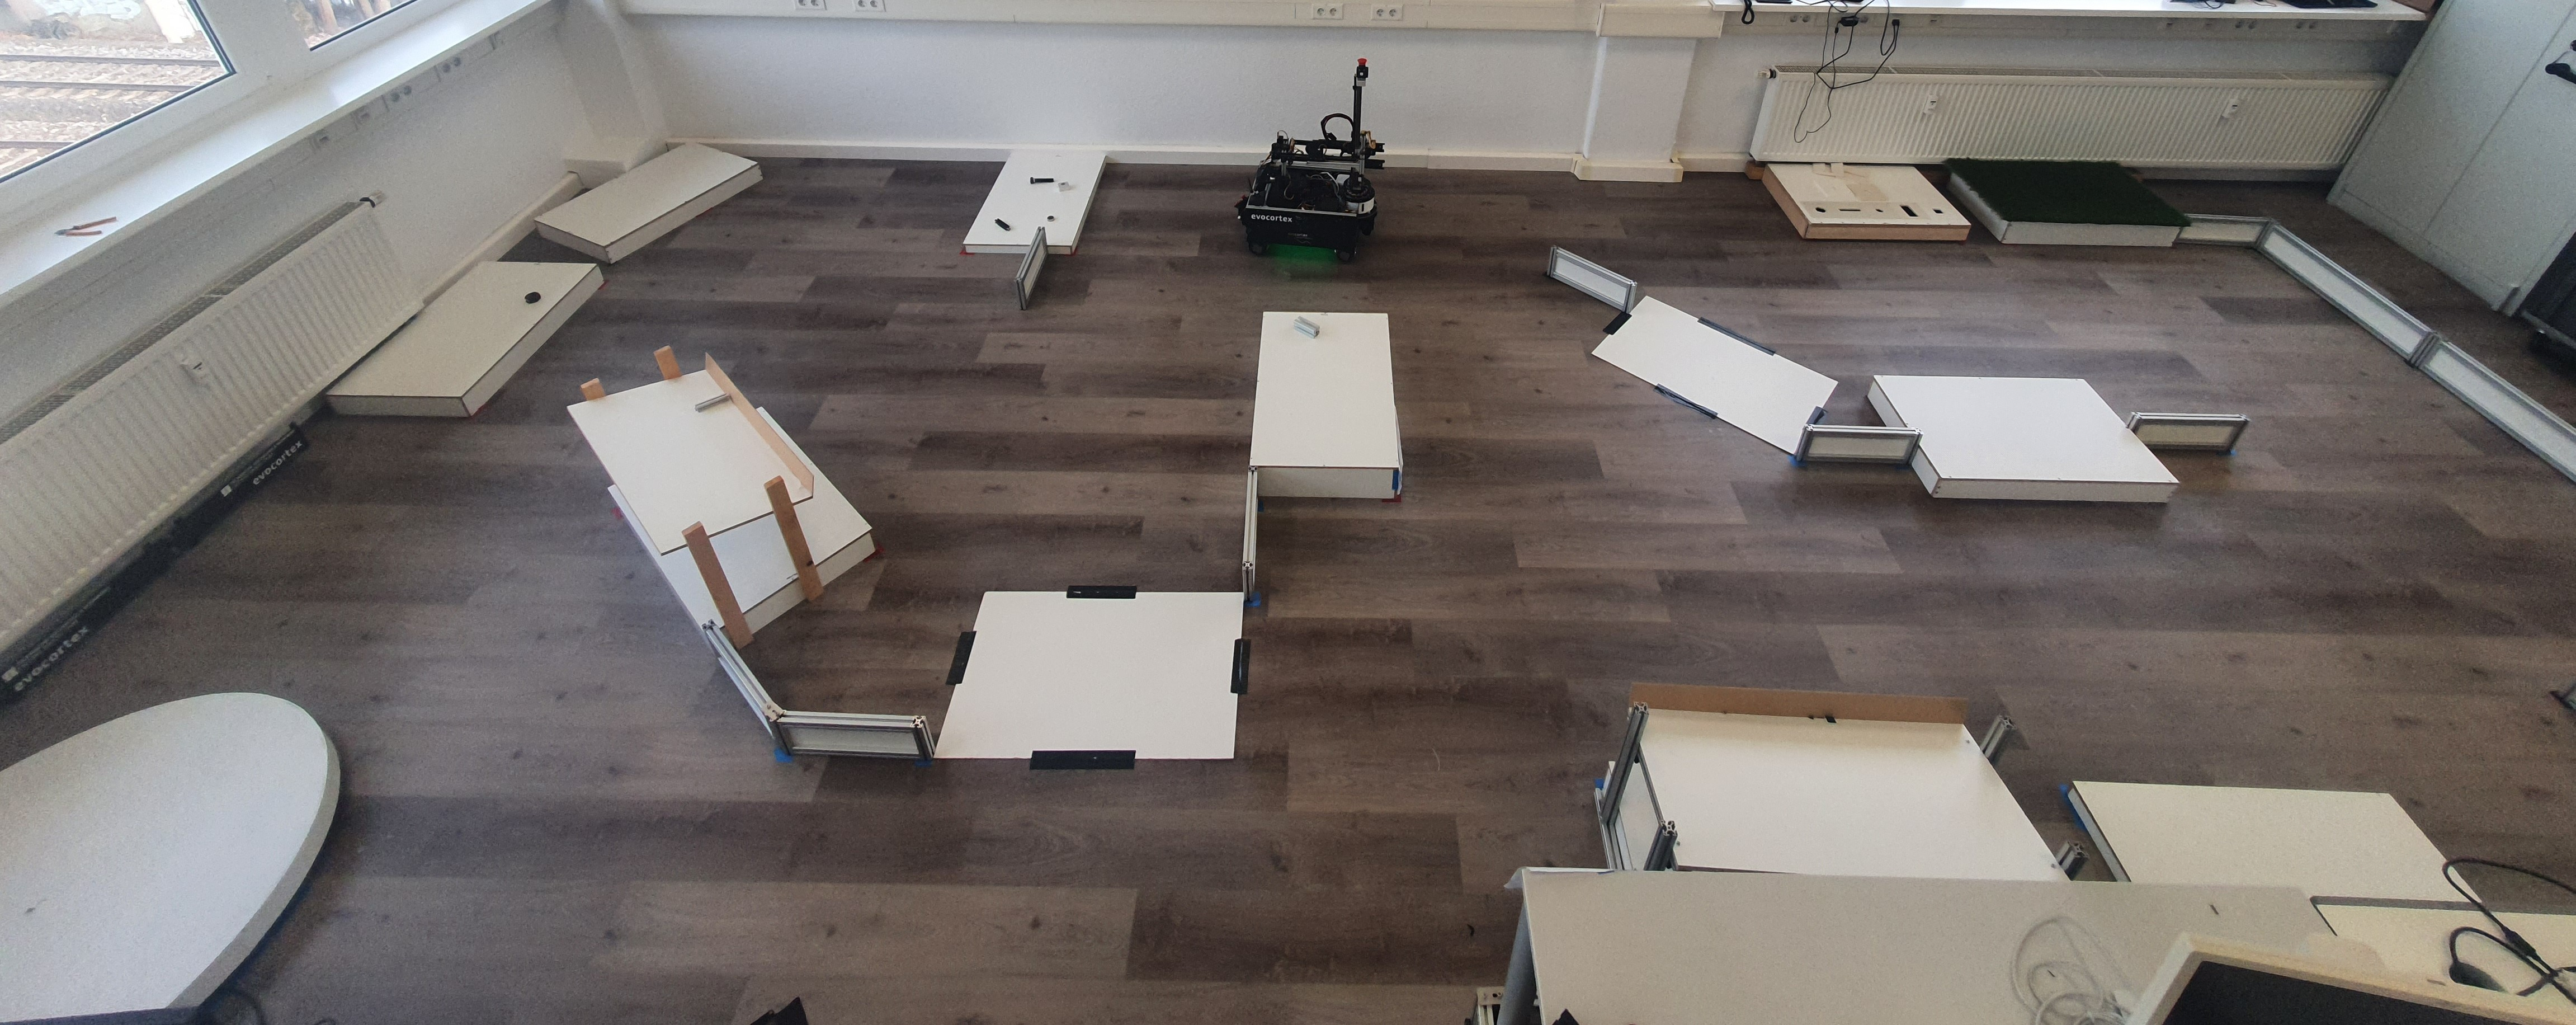
\includegraphics[width= \textwidth ]{./images/general_rules/arena_example.jpg}
\caption{An exemplary setup of a \RCAW environment.}
\label{fig:arena_example}
\end{figure}

Layouts may include rooms and hallways to create more realistic scenarios.
Service areas (see section \ref{ssec:serviceareas}) mark the locations for robots to perform tasks.
Each requested service area must be accessible via atleast one path of 80 cm width.

\begin{figure} [h!]
\centering
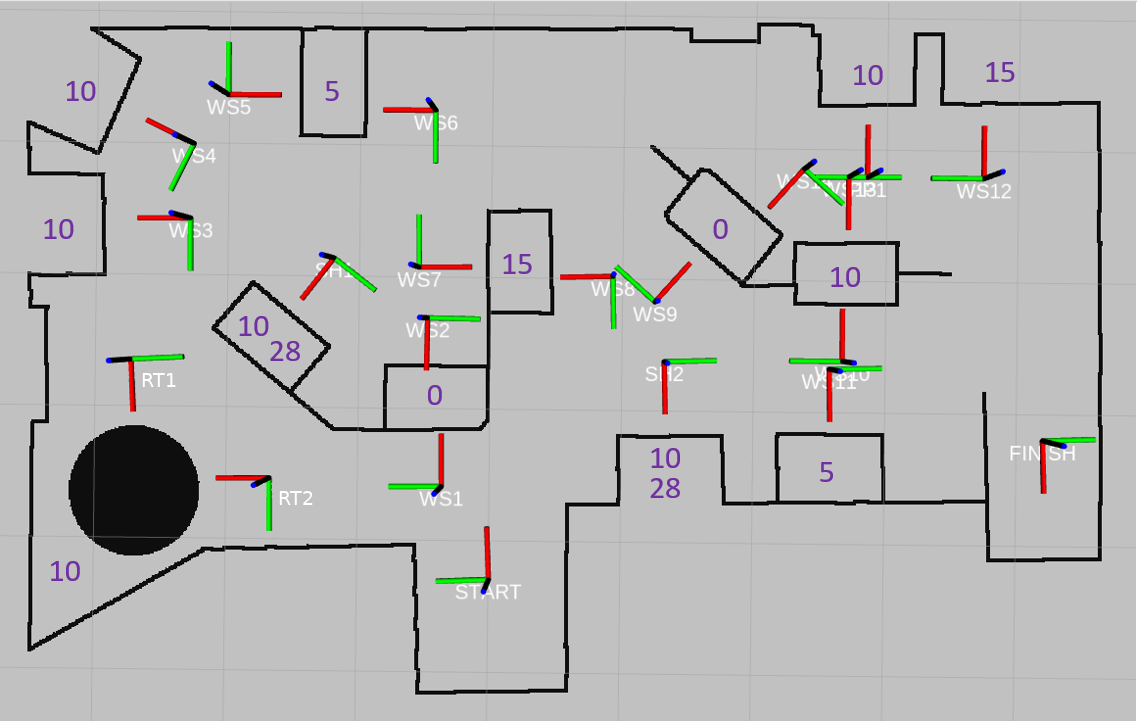
\includegraphics[width= 0.8\textwidth ]{./images/general_rules/arena_map_annotated}
\caption{Annotated 2D map of the environment in fig. \ref{fig:arena_example}}
\label{fig:arena_map_annotated}
\end{figure}

Each competition has a new and unique layout designed by the actual TC members.
It should feature:
\begin{itemize}
\item Area 10 m$^2$ - 120 m$^2$
\item Minimum distance between arena elements atleast 80 cm 
\item Widespread service areas entailing robot movements
\item Multiple paths between service areas
\item Start and Finish areas
\end{itemize}


\subsection{Service Areas} 
\label{subsec: serviceareas}

A service area indicates a location for a robot where tasks (e.g. picking or placing objects) have to be performed.
Such a location is usually a table with a flat white top (see fig. \ref{fig:arena_example}), but can also be a rotating table, shelf, precise placement station or any other type needed for a specific task.
In order to successfully reach a service area, robots must position themselves in front of the service area in a way that allows manipulation of the objects of interest. To enable robots to reach such a position, a rectangular area with 80 cm width must be kept free of obstacles (see fig. \ref{fig:arena_service_area_free}). 

\begin{figure} [h!]
\centering
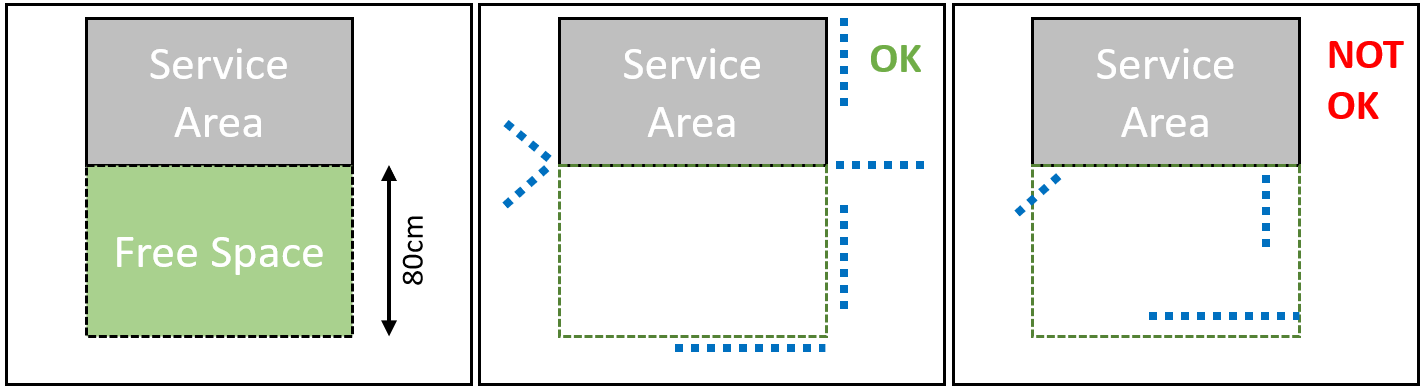
\includegraphics[width= 0.8\textwidth ]{./images/general_rules/arena_service_area_free_space}
\caption{Free Space in front of a service Area}
\label{fig:arena_service_area_free}
\end{figure}

The arena layout must define where the "front" of a table is.
Figure \ref{fig:arena_map_annotated} gives an example for the definition of the position of each service area, marking them as WSx (Workstation x), SHx (Shelf x) and CBx (Conveyor Belt x). The orientation only indicates the direction of the service area. It does not specify the robot's heading, which may be chosen by teams according to their individual robot design.

Tables that can be used from both sides (see fig. \ref{fig:arena_example}) are sometimes defined as two seperate workstations (e.g. WS5 \& WS6). However, manipulation of a service area requires the robot to have its center in the rectangular area defined in fig. XX TODO. This means that manipulation of the opposite service area is NOT allowed (see \ref{ssec:ManipulationZone}), even though it would be physically possible.

This rule also applies to the two positions for the rotating table (CB1 and CB2).
This makes smaller physical layouts possible that still provide the ability to create complex navigation challenges due to the amount of locations to visit.

Two special service areas are the START and FINISH positions. Both are rectangular areas for the robot to be positioned at the start or the end of a run. The service areas are marked using tape that may be crossed and are optionally equipped with light barriers used for time keeping.


\subsection{Walls and virtual Walls}
\label{subsec: Walls and virtual Walls}

The arena consists of outer and inner walls used to build structures, create obstacles or function as protection barriers for teams and viewers. Walls may be either physical (plank) or virtual (tape). Walls are infinitely height.
The arena is completely enclosed by walls (both types!), meaning robots are not allowed to exit the arena during a run. All types of walls are not changed during the competition.

The height of a physical wall must be not less than 20 cm and no more than 40 cm.
Most walls have a uniform main color (white), but may be enforced by metal (aluminum framework) and decorated with sponsor logos or ads.

Virtual walls are made of red and white tape (Tesa signal red/white) of 5 cm width. This tape may never be crossed during a run and is mainly used to close gaps in the physical outside walls.

\begin{figure} [h!]
\centering
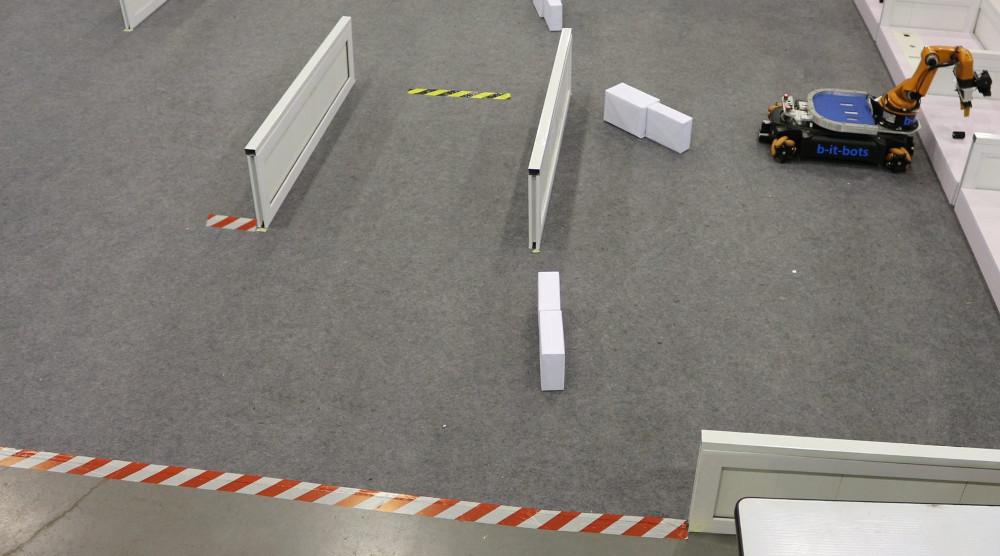
\includegraphics[width= 0.7\textwidth ]{./images/general_rules/barrier_tapes_in_china15.jpg}
\caption{Example of barrier tape used during \RC 2015. The red/white tape is used to indicate virtual walls , while the yellow/black one denotes a virtual fence.}
\label{fig:walls_and_virt_walls}
\end{figure}

Figure \ref{fig:walls_and_virt_walls} also shows black and yellow tape (Tesa signal black/yellow). 
This tape is referred to as 'Barrier Tape' and marks virtual fences. 
Such tapes are mainly used inside the arena to add obstacles.

\leander{i would clearly exclude barrier tape outside the arena}

\subsection{Obstacles}
\label{subsec: Obstacles}

In addition to the static arena elements, semi-dynamic obstacles may be placed inside the arena before a competition run begins. 
The position of such obstacles is decided by the referees during the setup phase of the run and randomized between different run types.

Obstacles may block paths partly or completely, as long as all active service areas are still reachable.
There are three main obstacle placement types:

\begin{itemize}
\item \textbf{Blocking:} 
A narrow section is completely blocked by the obstacle, which means that no robot can physically pass it ($<$ 20 cm).

\item \textbf{Semi-Blocking:} 
The obstacle reduces the distance between arena elements below the minimum width for a path. The path therefore counts as blocked, meaning that there must exist another valid path to all active service areas. Robots are still allowed to use all paths if they fit through the smaller gaps.

\item \textbf{Non-Blocking:}
The obstacle adds or enlarges an arena element but keeps all paths intact.
\end{itemize}

Obstacles can be either physical or virtual.
Physical obstacles measure atleast 2 x 2 x 20 cm (l x b x h) and may be made of any non-transparent, firm material (wood, metal). Some examples are bins, shipping boxes and wall elements. Their color is not specified.
All physical obstacles are treated like any other arena element during a run, including the rules for collisions.

Virtual obstacles are marked using the Barrier Tape from section \ref{subsec: Walls and virtual Walls}. 
These virtual fences recently have been introduced to the league, which is why collisions with them are treated differently (see REF SCORING).

\subsection{Arena Element Specifications}
\label{subsec: Arena Element Specifications}

\subsubsection{Markup Tape}
\label{subsubsec: Markup Tape}

Green electrical tape is considered as markup tape. This tape can be used everywhere, where it is useful. It is intended as a marker for the referees and teams and not for the robot. Therefore the color may deviate, but the color is not red or yellow to guarantee a clear difference to the other tapes. The tape is used to mark the start and goal area. Furthermore the tape can be used to mark the position of workstations (especially $0\,\text{cm}$) and walls. The latter ones are useful for restoring the arena in case of a major collision.

\subsubsection{Floor}
The floor is made of some firm material. Examples include floors made of concrete, screed, timber, plywood, chipboard, laminated boards, linoleum, PVC flooring, or carpet. Some examples are illustrated in Figure \ref{fig:example_floors}. Floors may neither be made of loose material of any kind (gravel, sand, or any material which may damage the functioning of the robot's wheels) nor may such material be used on top of the floor. Liquids of any kind are not allowed. The floor may have spots of unevenness of up to 1 cm in any direction (clefts, rifts, ridges, etc.).

\begin{figure} [h!]
	\begin{center}
		\subfloat{
\includegraphics[height = 2cm]{./images/general_rules/example_floor_1.jpg}} \hspace{0.1cm}
		\subfloat{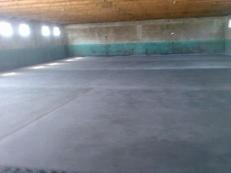
\includegraphics[height = 2cm]{./images/general_rules/example_floor_2.jpg}} \hspace{0.1cm}
		\subfloat{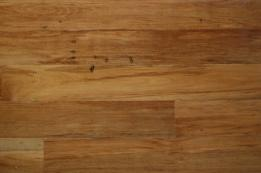
\includegraphics[height = 2cm]{./images/general_rules/example_floor_3.jpg}} \hspace{0.1cm}
		\subfloat{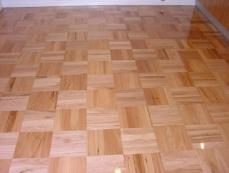
\includegraphics[height = 2cm]{./images/general_rules/example_floor_4.jpg}} \hspace{0.1cm}
		\subfloat{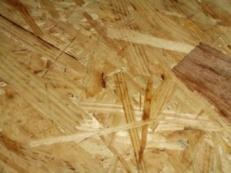
\includegraphics[height = 2cm]{./images/general_rules/example_floor_5.jpg}}\\
		\subfloat{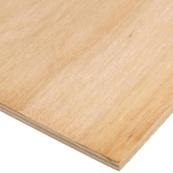
\includegraphics[height = 2cm]{./images/general_rules/example_floor_6.jpg}} \hspace{0.1cm}
		\subfloat{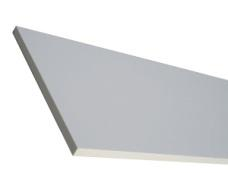
\includegraphics[height = 2cm]{./images/general_rules/example_floor_7.jpg}} \hspace{0.1cm}
		\subfloat{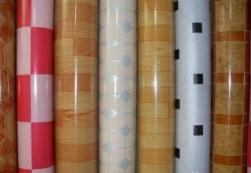
\includegraphics[height = 2cm]{./images/general_rules/example_floor_8.jpg}} \hspace{0.1cm}
		\subfloat{
\includegraphics[height = 2cm]{./images/general_rules/example_floor_9.jpg}} \hspace{0.1cm}
		\subfloat{
\includegraphics[height = 2cm]{./images/general_rules/example_floor_10.jpg}}
	\end{center}
	\caption{Examples of floors that can be used for \RCAW arenas.}
	\label{fig:example_floors}
\end{figure}


\subsubsection{Workstations - TODO}
\label{subsubsec: Workstations}

However, from 2020 on and in order to make the competition more realistic, the heights of the service areas will be variable, allowing the OC to adjust them before each test run. TODO...

If a service area has a height of zero cm, a green electrical tape (see \ref{subsubsec: Markup Tape}) will mark the area.
% (see Figure \ref{fig:barrier_tape_0cm}).
%The tape will be on the floor and will be blue/white striped.
A $0\,\text{cm}$-workstation can be active or inactive. Active means, that the current test (see \ref{sec:tests}) includes $0\,\text{cm}$-workstations.
If the workstation is active, the surrounded area may be covered by a white sheet of paper or thin wood. The material is not fixed.
The OC is responsible to replace it in case of pollution or tears. To reduce the tear, it is removed when the $0\,\text{cm}$-workstations are not active. If the floor is white or the workstation shall have an arbitrary surface, no cover needs to be installed.
$0\,\text{cm}$-workstations may be crossed, and does not count as a collision. If the laid out white surface is moved, it is not a collision.
If the robot touches a manipulation object while navigating, this will be handled as a collision. Examples for $0\,\text{cm}$-workstations are shown in figure \ref{fig:0cmws}.

\begin{figure} [h!]
	\begin{center}
		%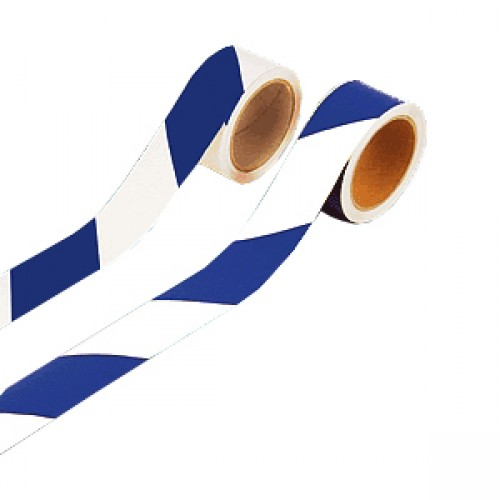
\includegraphics[height = 2.5cm]{./images/barrier_tape_0cm_area.jpg}
		\missingfigure[figwidth=6cm]{}	
	\end{center}
	\caption{$0\,\text{cm}$-workstations}
	\label{fig:0cmws}
\end{figure}

TODO:

Until 2017, service areas have always been represented by white coloured surfaces with no other decoy objects on it than the official ones in Tables \ref{tab:manipulation_objects} and \ref{tab:manipulation_objects_rockin}.
However, this does not represent real life scenarios.
The robot might have to pick objects from different colored or dirty places. Also there could be other industrial items on the surface area that the robot must avoid.
In order to make the operating environment more realistic, different kinds of arbitrary surfaces (Figure \ref{fig:ast_surface_example}) with decoy industrial items (Figure \ref{fig:ast_example}) have been introduced.
To facilitate the participation of newer teams that are yet focused on more basic functionalities, the integration of arbitrary surfaces is by now limited to:
\begin{itemize}
	\item One service area during the BTT1.
	\item Two service areas during the BTT2.
	\item Two service areas during the BTT3.
	\item Three service areas during the final round.
\end{itemize}

\begin{figure}[h!]
	\centering
	\subfloat[]{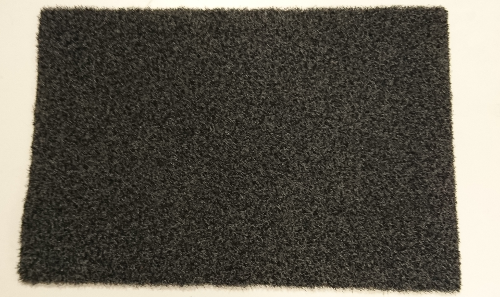
\includegraphics[width=.3\textwidth]{./images/Arbitrary_Surface_rug}}
	\hspace{0.5cm}
	\subfloat[]{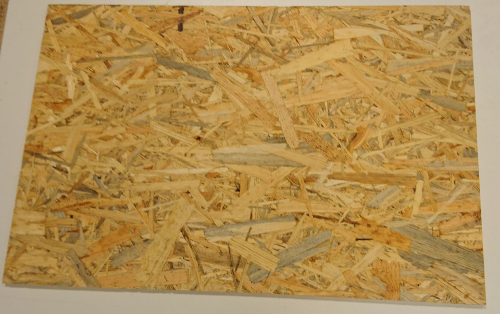
\includegraphics[width=.3\textwidth]{./images/Arbitrary_Surface_wood}}
	\hspace{0.5cm}
	\subfloat[]{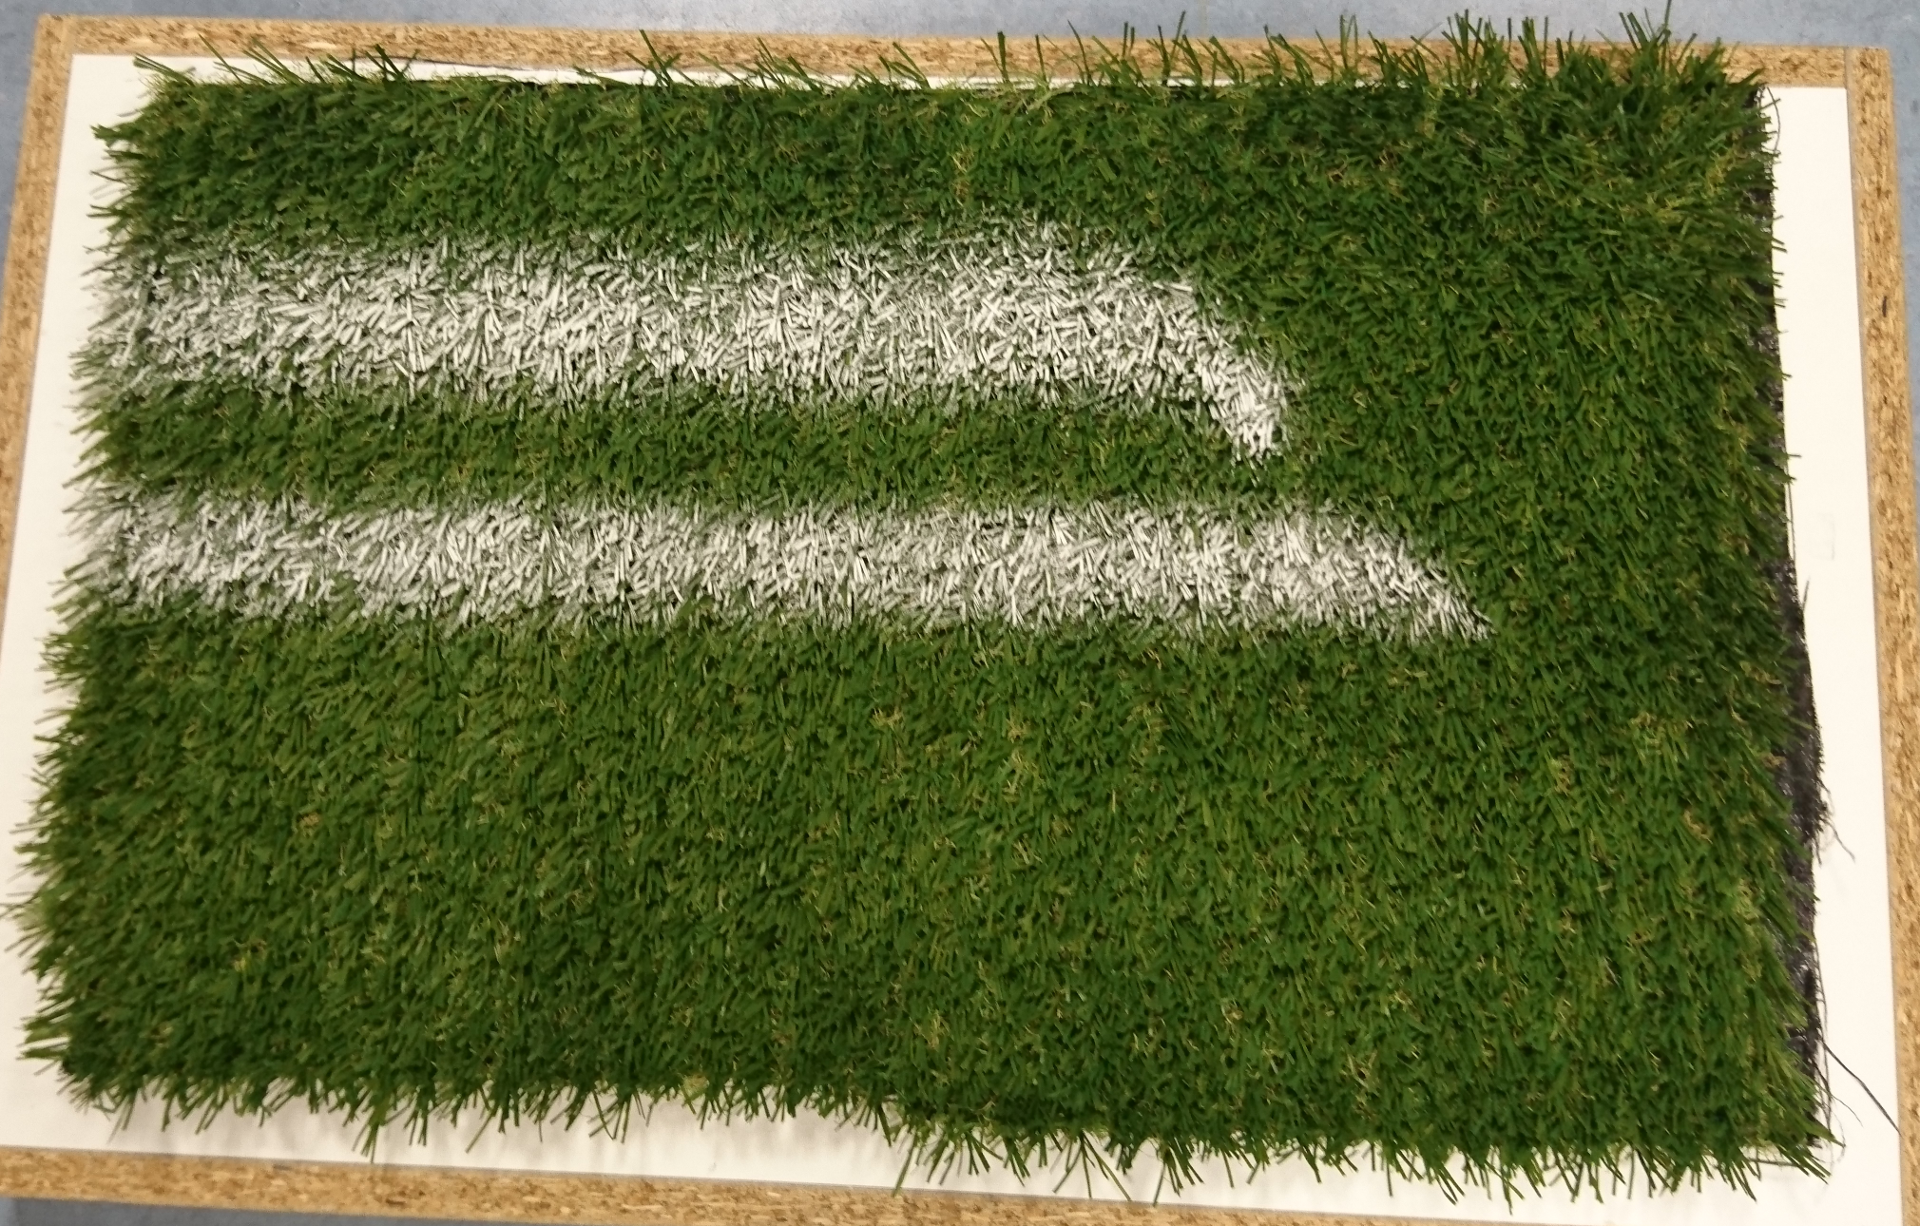
\includegraphics[width=.3\textwidth]{./images/Arbitrary_Surface_grass}}\\
	\subfloat[]{\includegraphics[width=.3\textwidth]{./images/Arbitrary_Surface_fake_wood_1}}
	\hspace{0.5cm}
	\subfloat[]{\includegraphics[width=.3\textwidth]{./images/Arbitrary_Surface_fake_wood_2}}
	\caption{Examples of arbitrary surfaces used for service areas.}
	\label{fig:ast_surface_example}
\end{figure}

\begin{figure}[h!]
	\begin{center}
		\subfloat[]{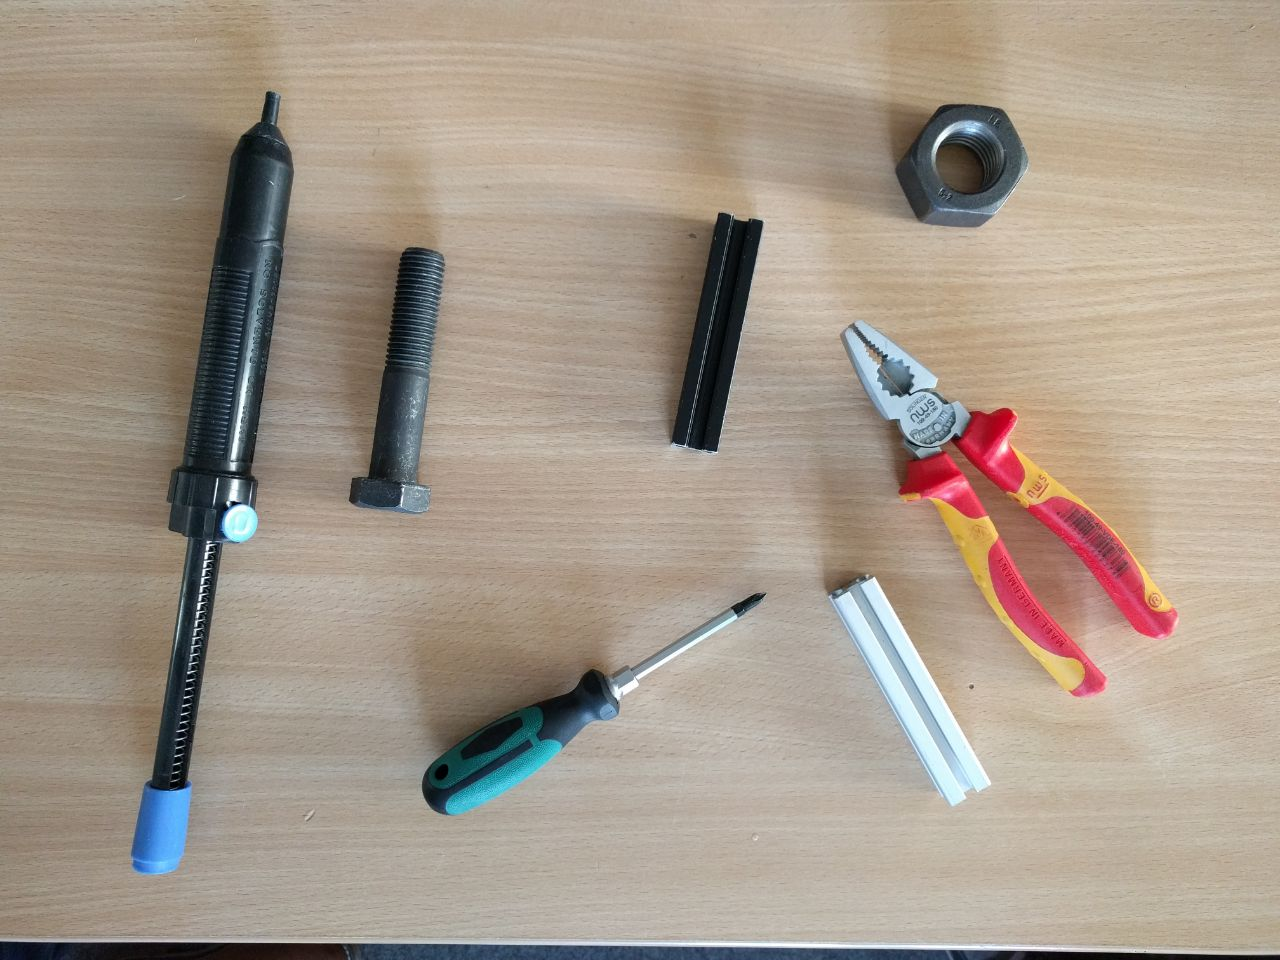
\includegraphics[height = \textwidth/3]{./images/realisticWorkingDeskI.jpeg}}
		\hspace{0.5cm}
		\subfloat[]{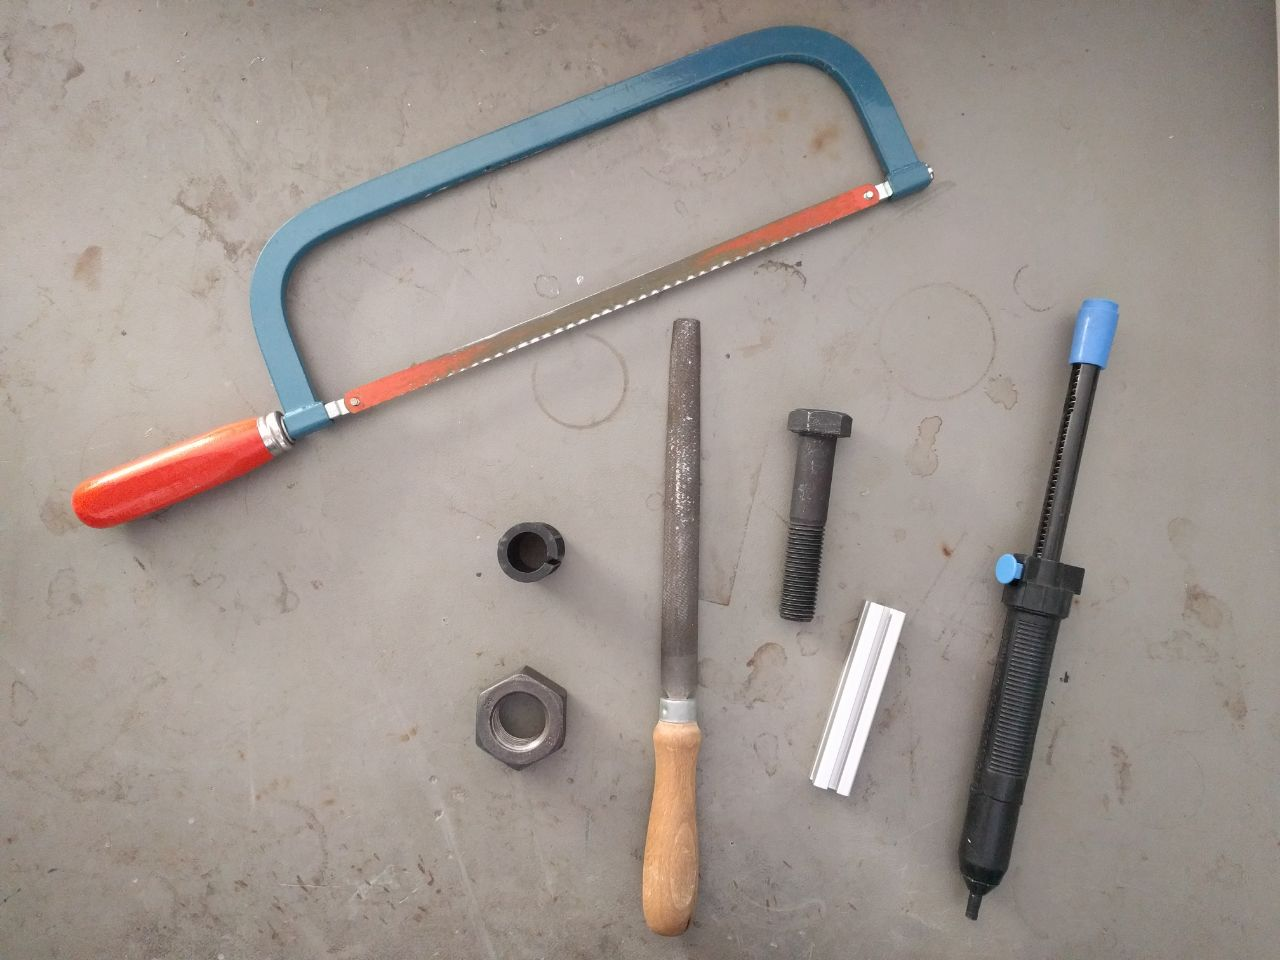
\includegraphics[height = \textwidth/3]{./images/realisticWorkingDeskII.jpeg}}
	\end{center}
	\caption{Examplary configuration of the working desks}
	\label{fig:ast_example}
\end{figure}

\subsubsection{Start and Goal Area}
\label{subsubsec: Start and Goal Area}

\leander{add new chapter, because there is currently no compact description of that}

One or two parts of the arena are separated with marking tape and considered as start and / or stop area. The start and stop area can be the same or two independent areas. The robot may leave the start area and enter the goal area only once. An area is leaved or entered when more than $50\%$ of the robot crossed the marking tape. In figure \ref{fig:tapeconfig} an exemplary tape configuration is shown.

\begin{figure} [h!]
	\begin{center}
		%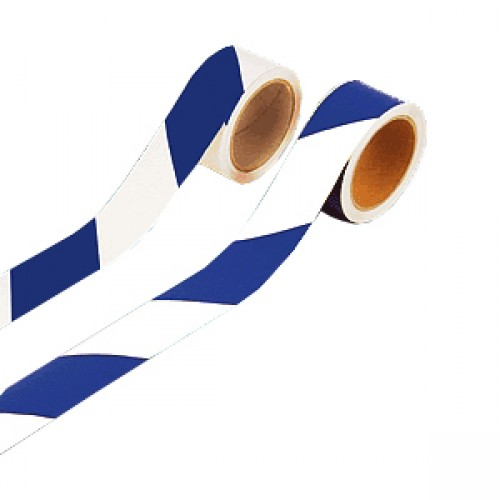
\includegraphics[height = 2.5cm]{./images/barrier_tape_0cm_area.jpg}
		\missingfigure[figwidth=6cm]{}	
	\end{center}
	\caption{tape configuraion, TODO...}
	\label{fig:tapeconfig}
\end{figure}


\subsection{Collisions}
\label{subsec: Collisions}

\leander{redudant to \ref{subsec: Tape collisions}}

For reasons of safety of people and property it is strictly unwanted for the robot to collide
with any of the environmental objects. Only collisions of the manipulator with the upside of
the service area are allowed. The different kind of collisions that can occur are defined in the
following subsections. Any Collisions cause a point penalty that is explained in section \ref{sec:ScoringAndRanking}. 

\textbf{Major Collision:}

If the robot (platform and arm) collides with a static element of the environment or touches a red white barrier tape it is considered as a major collision. If the manipulator cause a fundemental change of the environment at the service area it is counted as a major collision, this could be for example moving an arbitrary surface off the workspace. A major collision results in the termination of a run and the arena can be restored. 

\textbf{Minor Collision:}

If the manipulator collides with an interaction element of the arena (RTT, PPT Cavities, upper level
of Shelf) it is considered a minor collision. The only exception is the collision of the manipulator
of the robot with the surface of the manipulation area.

\textbf{Tape Collision:}

Red/White Tape: 
This tape represents a virtual wall with an infinite height. This wall shall not be crossed. If any part of the robot (including the manipulator and gripped object; excluding cables) is above the tape, it is considered as a major collision. The idea behind this is, that virtual walls are like real walls and only replaced by tape to increase the visibility for the referees and spectators.

Yellow/Black Tape: 
This tape is called Barrier Tape and represents a virtual fence. If any
part of the robot touches a barrier tape, it is considered as a Barrier Tape Collision. Barrier
Tape collision induce a point penalty proportional to the final points of the run. With
each collision 5\% of the final points are deducted up to a maximum of 20\%. For beginner
teams the option exists to opt-out of Barrier Tape and take a static deduction of 15\% of
the final points of the run.


%\subsection{Racks}
%Service areas, e.g. loading and unloading areas, may foresee the use of racks. Objects to be delivered or removed from racks have to be placed or picked up from the top. The height of the racks should be not lesser than 5 cm and not more than 40 cm. The color for the top surface of racks is a bright uniform color such as white or light gray, unless a test specifies a different color. The top surface of the rack may be specially designed in order to serve specific purposes, e.g. holding objects.


\subsection{Shelves}\label{sec:Shelves}
In Basic Transportation Test three and the final runs (BTT3 in \ref{sec:Basic Transportation Test}, finals \ref{sec:Final}) Service areas may foresee the use of shelves and shelf units as depicted in Figure~\ref{fig:shelf}. 

Objects to be delivered or removed from shelves have to be placed or picked sideways. The height of the shelves should be not lesser than 5 cm and not be more than 40 cm.

The workspace on the bottom shelf is considered like a standard workspace on a $10\si{\centi\meter}$ table. The first $15 \si{\centi\meter}\pm 2\si{\centi\meter} $ has not to be covered by the top shelf. 

The top shelf surface may be specially designed in order to serve specific purposes, e.g.\, holding objects. Objects to pic up are always placed on the bottom shelf, during the competition a placement of a delivered object has to be done on the top shelf.  

\begin{figure}[h!]
\centering
\subfloat[A shelf with two levels and uniform colored surfaces.]{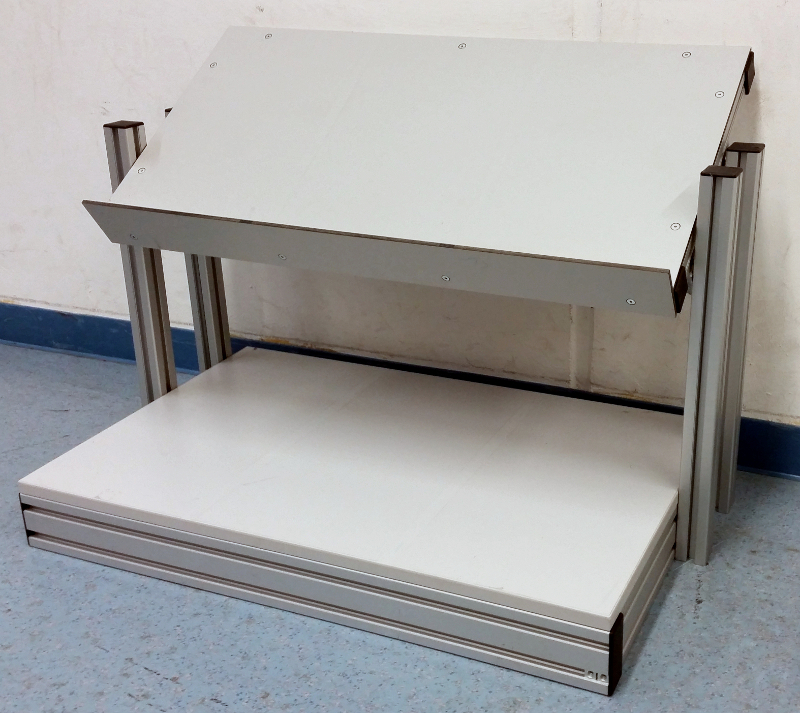
\includegraphics[width=0.4\textwidth ]{./images/shelf.jpg}}
\hspace{0.5cm}
\subfloat[Technical draw of shelf configuration.]{ 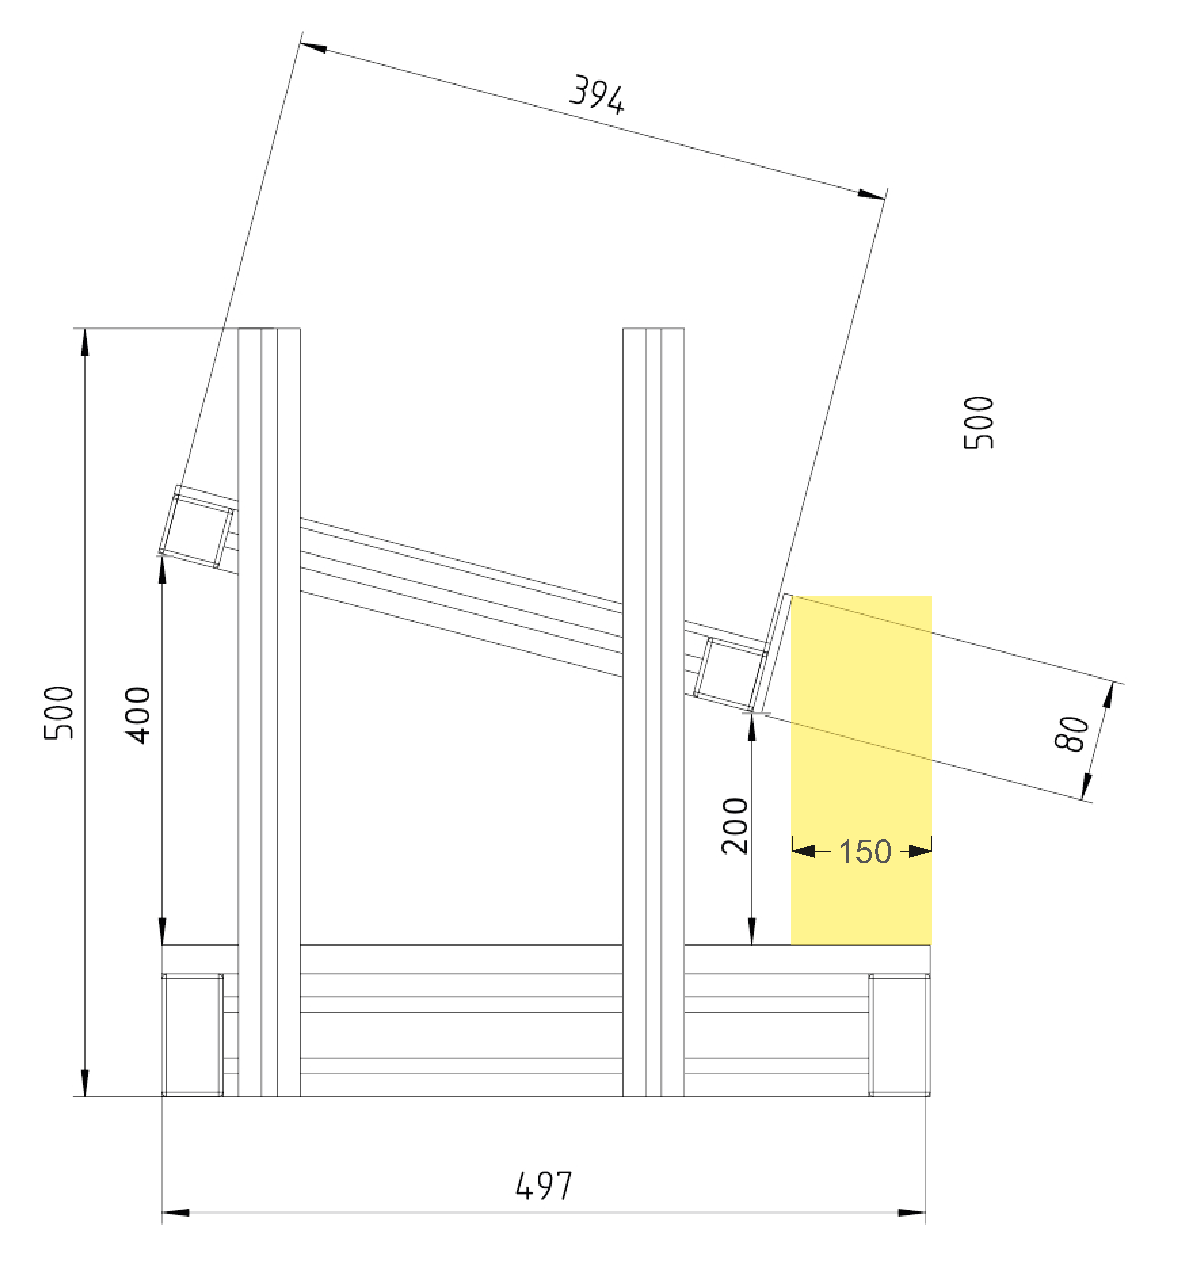
\includegraphics[width=0.4\textwidth ]{./images/shelfUpdate.pdf} }
\caption{Exemplary shelf and generic technical drawing.}%
\label{fig:shelf}
\end{figure}


\subsection{Rotating Table}\label{sec:Rotating Table}
\martin{minimum and maximum speed has to be discussed}
For the Rotating Table Test (RTT in Section~\ref{sec:Rotating Table Test}) a rotating table as depicted in Figure~\ref{fig:rottable} is used. 
Objects to be removed from the table have to be placed with a boarder of $2\si{\centi\meter}$ in a so defined grasp region. The height of the table should be not lesser than $8\si{\centi\meter}$ and not be more than $12\si{\centi\meter}$. The diameter of the table should be not lesser than $50\si{\centi\meter}$ and not more than $100\si{\centi\meter}$. The table has to have a white surface colour. The rotating speed of the table depends on the diameter. The objects speed should be able to vary between $0.2 \si{\meter\per\second} \le v_{object} \le 0.5 \si{\meter\per\second}$ and has to be adjusted by the referees before a team starts its run to a fixed value. This is changed after each run to another random chosen value in this range. During the run of a team the speed is static. Example: For a table with diameter $d_{table}=1\si{\meter}$, objects are placed on a grasp region with the diameter $d_{object}=0.8\si{\meter}$ with $\omega_{table} = \frac{2 \cdot v_{objects} }{d_{grasp}}=\frac{2 \cdot 0.2}{0.8}=0.5\si{\radian\per\second}$ and with $n_{table}=\frac{\omega_{table}}{2 \cdot \pi}=\frac{0.5}{2 \cdot \pi}$ the minimum rotational speed of the table $n_{table}= 0.0796 \si{\per\second}$ (rounds per second) can be calculated.  

\begin{figure}[h!]
	\centering
	\subfloat[A rotationg table with some objects.]{%
		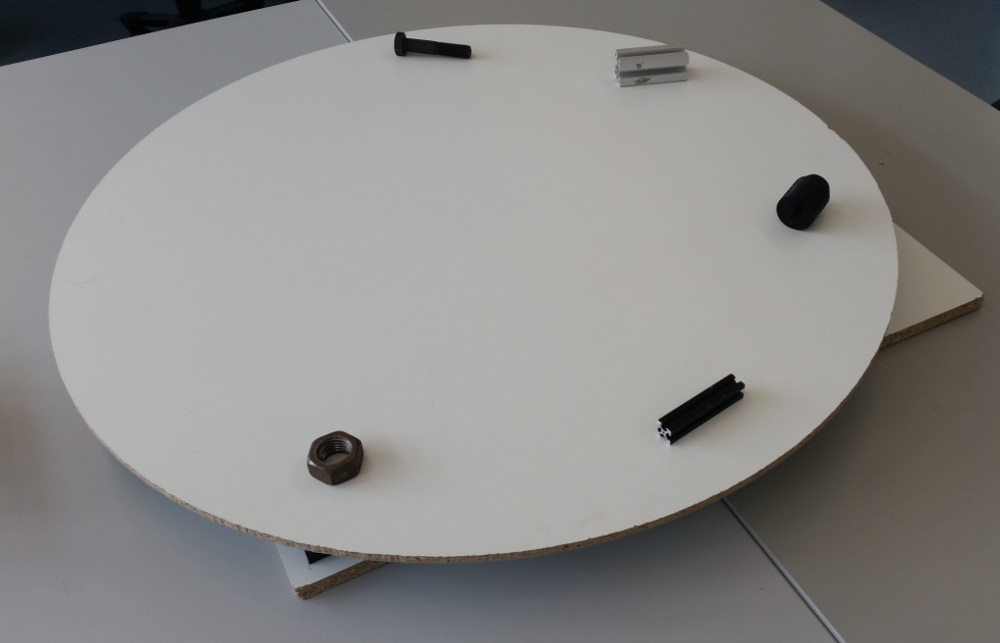
\includegraphics[width=0.4\textwidth,angle=0 ]{./images/rotating_table.jpg}%
	}%
	\subfloat[Technical draw of rotating table.]{%
		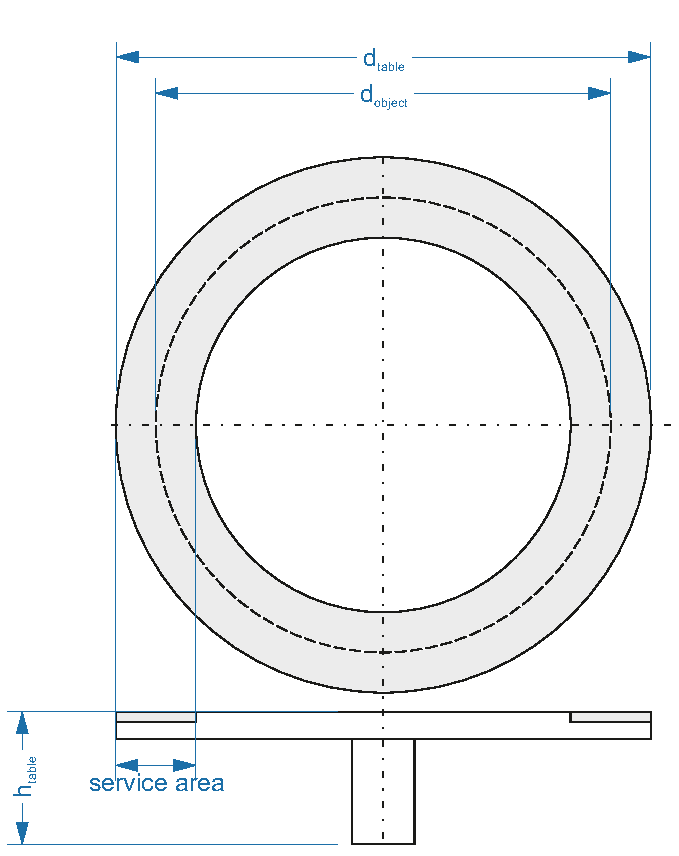
\includegraphics[width=0.4\textwidth ]{./images/rotating_table_schematic.pdf}
	}
	\caption{Exemplary rotating table and generic technical drawing.}%
	\label{fig:rottable}
\end{figure}


\section{Design of Navigation Tasks} \label{sec:NavigationTasks}
Every task has some navigation involved in it. Successful navigation will be awarded in every test according to Table \ref{tab:InstancePoints}. If not defined differently in the respective test, a navigation is successful when the robot reached the service area as defined in section \ref{ssec:Navigating}. 

\textbf{REMARK:} Since 2020 the BNT test is removed from the set of tests done at the competition. Remark that points for reaching service areas are given in all tests, so that teams which are only able to navigate with their robot can still achieve points in all tests.


\subsection{Reaching a Service Area} \label{ssec:Navigating}
A service area counts as successfully reached if the robot would be able to manipulate the service area it is standing on. The manipulation range will be subjectively evaluated by the referees.


\section{Design of Manipulation Tasks} \label{sec:ManipulationTasks}


\subsection{Manipulation Zone} \label{ssec:ManipulationZone}
The manipulation zone defines the area where objects can be placed. Thereby, the following constraints need to be satisfied:
\begin{itemize}
	\item The maximum depth of the manipulation zone is 20 cm.
	\item The minimum distance between objects to each other is 2 cm.
	\item The minimum distance of the beginning of the manipulation zone to a wall is 10 cm.
	\item There as an offset of 2 cm from the border of the service area to the manipulation zone.
\end{itemize}
Note, the constraints do not permit, that objects can be partially occluded dependent on the viewpoint.
\begin{figure} [h!]
\centering
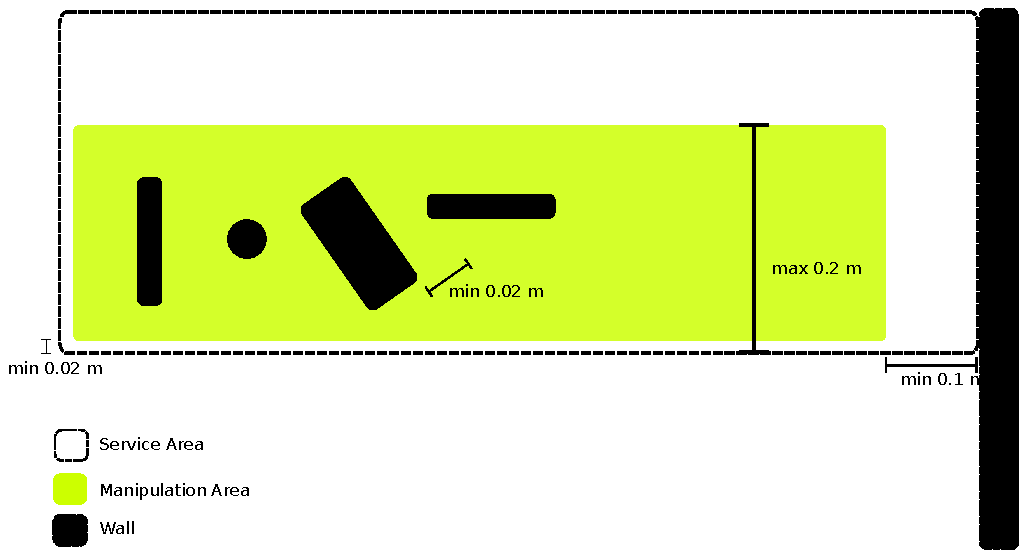
\includegraphics[width=1.0\textwidth ]{./images/manipulation_zone.pdf}
\caption{Manipulation zone: the green color indicates the area where objects can be placed on a service area by the referees.}
\label{fig:manipulation_zone}
\end{figure}


\subsection{Manipulation Objects} \label{ssec:ManipulationObjects}
The manipulation objects in \RCAW shall include a wide range of objects relevant in industrial applications of robotics. They eventually cover any raw material, (semi-)finished parts or products as well as tools and possibly operating materials required for manufacturing processes.
\par

The intention is to start with a simple set of objects of different shapes and colors. Every year, the spectrum shall then be widen in at least one aspect. 
The initial set of objects includes basic standard screws and nuts with various sizes and masses as well as so called rocking objects as shown in Table~\ref{tab:manipulation_objects} and Table~\ref{tab:manipulation_objects_rockin}. Objects of one kind can slightly vary e.g. considering the surface and coating colour. 
Rocking objects are spare parts from the KUKA you-bot platform often used in the competition, due to the fact that the KUKA you-bot and the rocking objects are not longer produced in future those objects will be replaced with other standard parts used in industry. 

\textbf{REMARK:} In 2022 teams has the option to use a set of original rocking objects or a set of 3D printed rocking objects. The set of 3D printed objects has to be printed in standard grey/silver colour using fine quality settings and PLA as printing material. An example is given with PLA Silver, RAL number 9006, thickness 1.75 or 2.85, not specified in detail (\href{https://www.amazon.de/dp/B07F44HYL6/ref=cm_sw_em_r_mt_dp_T9K6ARS1AHSMBR2B6SPS  }{example material from amazon}). Figure~\ref{fig:rocking_printed} shows an example of all rocking objects printed with a fused filament fabrication (FFF) 3D printer. 

For the placement of manipulation objects the following terms are used:

\begin{itemize}
\item Position: point within 2D coordinate system of a service area,
\item Rotation: rotation around vertical axis of a service area,
\item Orientation: rotation around horizontal axes of a service area, i.e. whether the object is standing upright or lying on its side
\item Pose: combination of position, rotation and orientation.
\end{itemize}

\newcommand{\imageView}[1]{\includegraphics[width=2cm, valign=c]{#1}}
{
\newcommand{\rowpadding}{0.4cm}
\setlength\extrarowheight{\rowpadding}
\begin{table}[p]

\begin{tabular}{|c|c|c|m{8cm}|}
\hline
Object & Symbolic Description & Mass & Details \\
\hline

\imageView{./images/F20_20_B.jpg} & \texttt{F20\_20\_B} & 49 g & Small aluminium profile \newline
 Coating/Colour: black anodized\newline
 Height: 20 mm \newline
 Width: 20 mm \newline
 Length: 100 mm \\ [\rowpadding]
\hline

\imageView{./images/F20_20_G.jpg} & \texttt{F20\_20\_G} & 49 g & Small aluminium profile \newline
 Coating/Colour: gray anodized\newline
 Height: 20 mm \newline
 Width: 20 mm \newline
 Length: 100 mm \\ [\rowpadding]
\hline

\imageView{./images/S40_40_B.jpg} & \texttt{S40\_40\_B} & 186 g & Big aluminium profile\newline
 Coating/Colour: black anodized\newline
 Height: 40 mm \newline
 Width: 40 mm \newline
 Length: 100 mm \\ [\rowpadding]
\hline

\imageView{./images/S40_40_G.jpg} & \texttt{S40\_40\_G} & 186 g & Big aluminium profile \newline
 Coating/Colour:  gray anodized\newline
 Height: 40 mm \newline
 Width: 40 mm \newline
 Length: 100 mm \\ [\rowpadding]
\hline
\imageView{./images/M20_100.jpg} & \texttt{M20\_100} & 296 g & Screw\newline

 ISO4014, DIN 931, CSN 021101, PN 82101, UNI 5737, EU 24014 \newline
 Coating/Colour: blank, black burnished \newline
 Size: M$20\times 100$ \\ [\rowpadding]
\hline
\imageView{./images/M20.jpg} & \texttt{M20} & 56 g & Small nut\newline

 ISO4032, DIN934,  CSN 021401, PN 82144, UNI 5588, EU 24032  \newline
 Coating/Colour: blank, black burnished \newline
 Size: M20 \\ [\rowpadding]
\hline
\imageView{./images/M30.jpg} & \texttt{M30} & 217 g & Big nut\newline

 ISO4032, DIN934,  CSN 021401, PN 82144, UNI 5588, EU 24032  \newline
 Coating/Colour: blank, black burnished \newline
 Size: M30 \\ [\rowpadding]
 \hline
\end{tabular}
\caption{\RCAW manipulation object set.}
\label{tab:manipulation_objects}
\end{table}


\begin{table}[p]
\begin{tabular}{|c|c|c|m{6cm}|}
\hline
Object & Symbolic Description & Mass & Details \\
\hline

\imageView{./images/bearingBoxA.jpg} & \texttt{Bearing\_Box} & 102 g & Bearing box\newline
 Height: 25 mm \newline
 Width: 45 mm \newline
 Length: 50 mm \newline
 Inner diameter: 32 mm \\ [\rowpadding]
\hline

\imageView{./images/bearing.jpg} & \texttt{Bearing} & 42 g & Bearing\newline
 Height: 13 mm \newline
 Inner diameter: 15 mm \newline
 Outer diameter: 32 mm \\ [\rowpadding]
\hline

\imageView{./images/axis.jpg} & \texttt{Axis} & 40 g & Axis\newline
 Diameter: 27 mm \newline
 Length: 96 mm \\ [\rowpadding]
\hline

\imageView{./images/distanceTube.jpg} & \texttt{Distance\_Tube} & 5 g & Distance tube\newline
 Height: 10 mm \newline
 Inner diameter: 28 mm \newline
 Outer diameter: 32 mm \\ [\rowpadding]
\hline

\imageView{./images/motor.jpg} & Motor & 20 g & Motor\newline
 Diameter: 42 mm \newline
 Length: 87 mm \\ [\rowpadding]
\hline
\imageView{./images/R20.jpg} & \texttt{R20} & 14 g & Plastic tube\newline
Inner diameter: 20 mm \newline
Outer diameter: 30 mm \newline
Length: 45 mm \\ [\rowpadding]
\hline
%\imageView{./images/V20.jpg} & \texttt{V20} & 14 g & Inner diameter: 20 mm \newline
%Outer diameter: 30 mm \newline
%Length: 45 mm \\
%\hline
\end{tabular}
\caption{RoCKIn manipulation object set.}
\label{tab:manipulation_objects_rockin}
\end{table}
}


\begin{figure}[h!]
	\begin{center}
		\subfloat[]{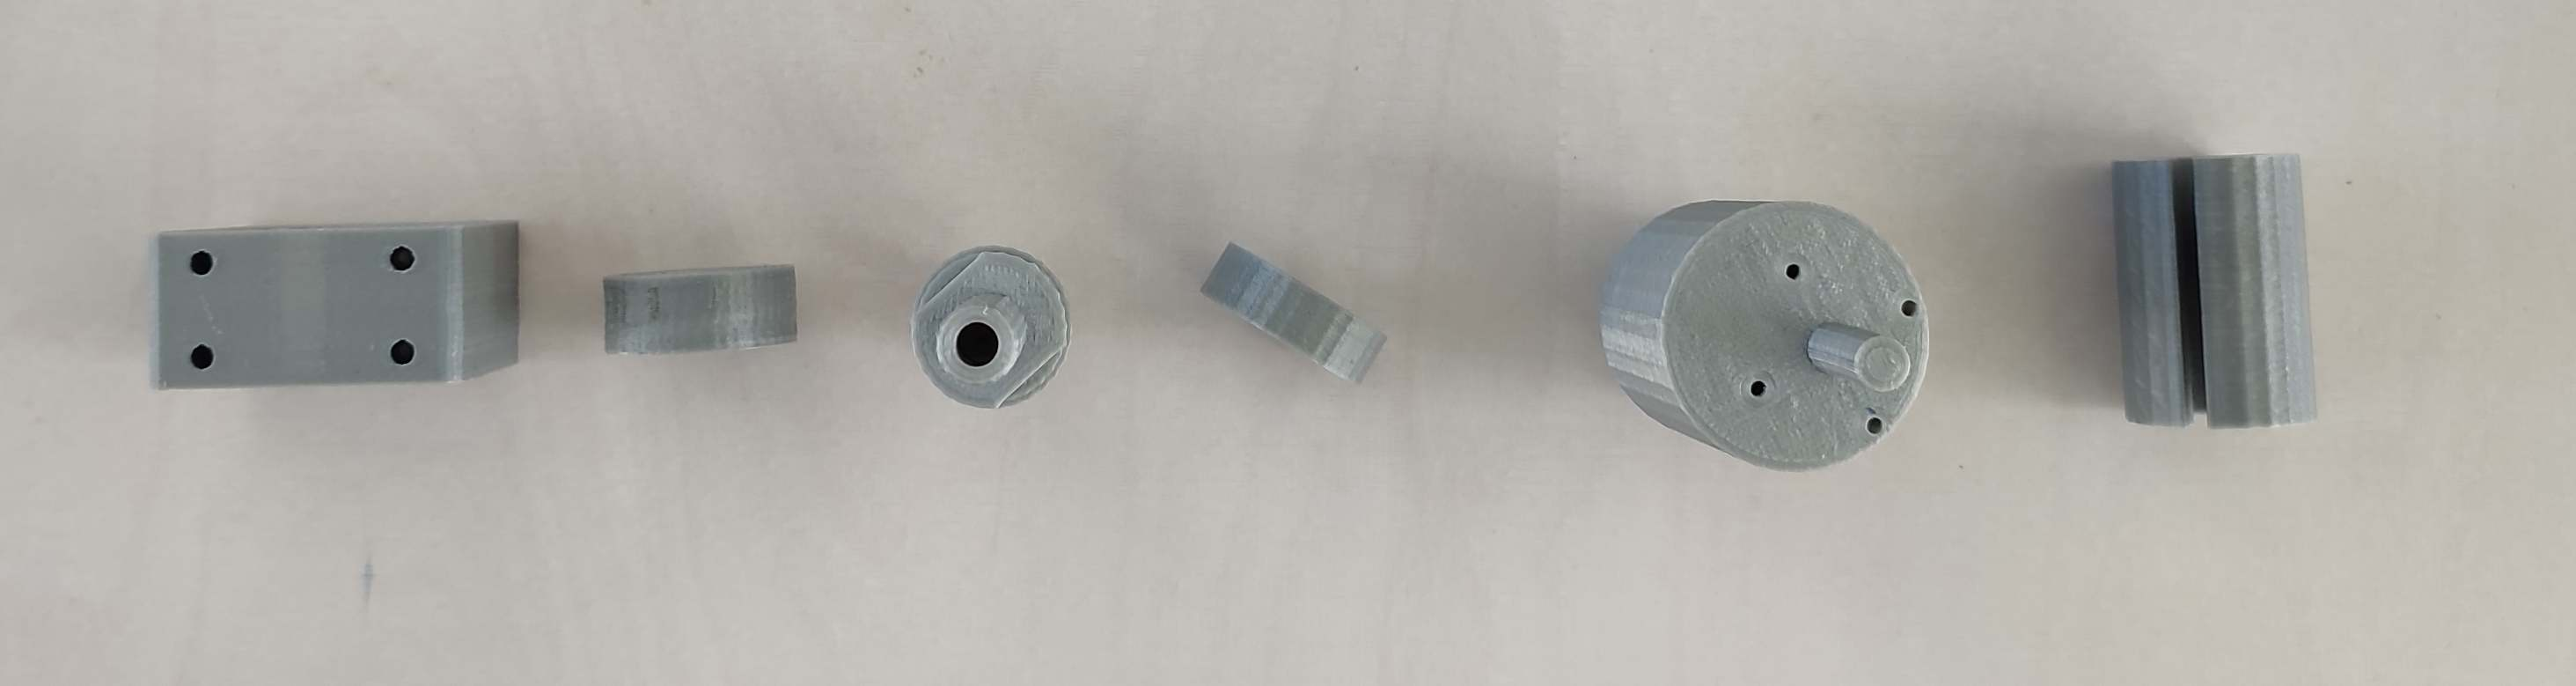
\includegraphics[width=\textwidth]{./images/rockingPrinted1.jpg}}
		\vspace{0.5cm}
		\subfloat[]{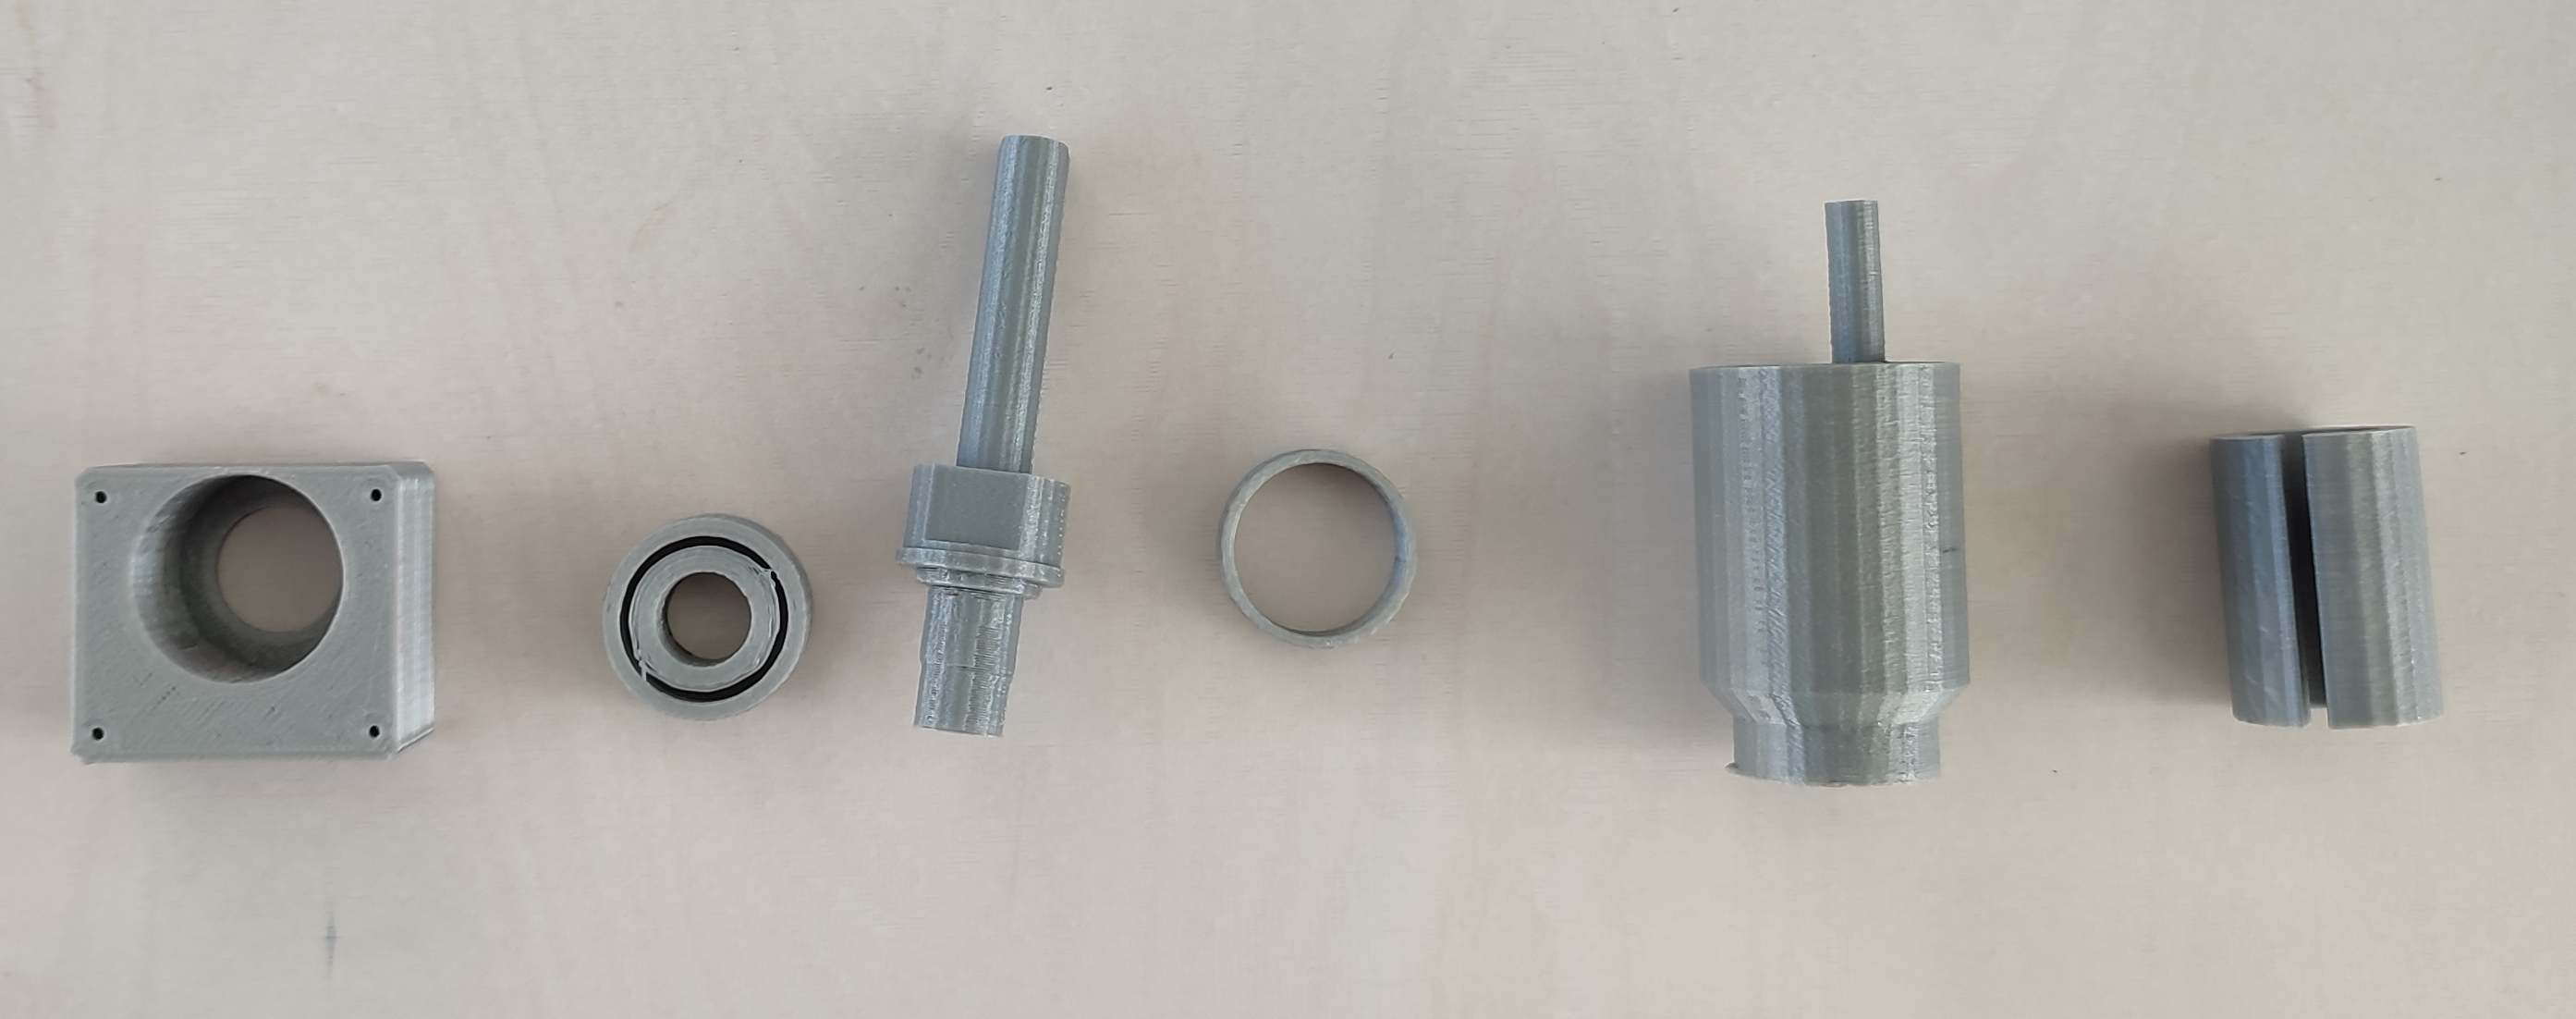
\includegraphics[width=\textwidth]{./images/rockingPrinted2.jpg}}
	\end{center}
	\caption{Examplary 3D printed rocking objects (bearing box, bearing, axis, distance\_tube, motor, plastic tube R20). Material:  PLA silver, 2.85mm. Printer: Ultimaker 3 extended. Printer settings: fine}
	\label{fig:rocking_printed}
\end{figure}

\textbf{REMARK: THIS OBJECTS ARE JUST EXAMPLES, NOT FINAL! } In 2023 a new set of objects will be introduced. Therefore standardised mechatronic components will be used some examples are shown in Table~\ref{tab:new_objects}.  

\begin{table}[h!]
	\begin{tabular}{|m{2cm}|c|c|m{8cm}|}
		\hline
		Object & Symbolic Description & Mass & Details \\
		\hline
		\imageView{./images/newObjects/welle3d.jpg} \newline
		\imageView{./images/newObjects/welleSchematic.jpg}
		
		& \texttt{Axis2} & 180 g & Steel axis \newline
		Misumi: SFUB25-25-F28-P17-T15-S10-Q20 \newline
		Coating/Colour: blank, black burnished \newline
		Length: 68 mm \newline
		Diameter: 17mm, M20 \newline
		see Figure~\ref{fig:welle2Schematic} \newline
		\href{https://de.misumi-ec.com/vona2/detail/110302635710/?CategorySpec=00000146753%3a%3ab%2cc}{Misumi}\\
		\hline
		
		\imageView{./images/newObjects/bearing2.jpg} & \texttt{Bearing2} & 100 g & Bearing \newline 
		SKF YAR203-2F\newline
		Coating/Colour: gray \newline
		Useable with housing\newline
				\href{https://www.skf.com/sg/products/rolling-bearings/ball-bearings/insert-bearings/productid-YAR%20203-2F}{SKF}\\
		\hline
		
		\imageView{./images/newObjects/housing.jpg} & \texttt{Housing} & 60 g & Housing \newline 
		SKF P40\newline
		Coating/Colour: gray \newline
		Useable with bearing\newline
				\href{https://www.skf.com/sg/products/mounted-bearings/ball-bearing-units/pillow-block-ball-bearing-units/productid-P%2040}{SKF}\\
		\hline
		
		\imageView{./images/newObjects/motor.jpg} & \texttt{Motor2} & 350g & Motor 755\newline
		Coating/Colour: gray \newline
		Size: $66.7 \times 42.0 \si{\milli\meter}$\newline
		Diameter: $d_{axis}=5\si{\milli\meter}$, $l_{axis}=10\si{\milli\meter}$ \newline
				\href{https://www.amazon.de/EsportsMJJ-12V-36V-3500-9000Rpm-Drehmoment-Hochleistungsmotor/dp/B075D85KVV}{Amazon}\\
		\hline
				
		\imageView{./images/newObjects/FlangedResinCollar.jpg} & \texttt{Spacer} &  & Flanged Spacer\newline
		Misumi CLJHJ25-30-70  \newline
		Coating/Colour: white \newline
		Size: $70\si{\milli\meter}$\newline
		Diameter: $d_{inner}=25\si{\milli\meter}$, $d_{outer}=30\si{\milli\meter}$ \newline
		\href{https://us.misumi-ec.com/vona2/detail/110300236450/?curSearch=%7b%22field%22%3a%22%40search%22%2c%22seriesCode%22%3a%22110300236450%22%2c%22innerCode%22%3a%22%22%2c%22sort%22%3a1%2c%22specSortFlag%22%3a0%2c%22allSpecFlag%22%3a0%2c%22page%22%3a1%2c%22pageSize%22%3a%2260%22%2c%2200000042362%22%3a%22mig00000001500952%22%2c%2200000042368%22%3a%22b%22%2c%22jp000157843%22%3a%22mig00000000344081%22%2c%22jp000157846%22%3a%22mig00000001417174%22%2c%22jp000157851%22%3a%22mig00000000344088%22%2c%2200000334029%22%3a%2230%22%2c%2200000334032%22%3a%2270%22%2c%22typeCode%22%3a%22CLJHJ%22%2c%22fixedInfo%22%3a%22MDM0000085422111030023645020110476153310093415426696895%7c14%22%7d&Tab=preview}{Misumi}\\
		\hline
\end{tabular}
	\caption{\RCAW New set of manipulation objects.}
	\label{tab:new_objects}
\end{table}

\begin{figure}[h!]
	\begin{center}

\includegraphics[width=\textwidth]{./images/newObjects/welleSchematic.jpg}
	\end{center}
	\caption{Schematic drawing of new manipulation object Axis2. Made of steel, blank or black burnished.}
	\label{fig:welle2Schematic}
\end{figure}




\subsection{Containers}
As in many industrial settings, the \RCAW environment may be equipped with several containers (see Figure~\ref{fig:containers}). The containers are defined as industrial plastic stacking boxes size 2B, outer dimensions: $135 \times 160 \times 82  \si{\milli\meter}$, usable dimensions: $120 \times 125 \times 65  \si{\milli\meter}$  in red and blue (\href{https://www.amazon.de/gp/product/B0062TUUOE/ref=ppx_yo_dt_b_asin_title_o01_s00?ie=UTF8&psc=1}{example container from amazon}). 
They can store any kind of manipulation object defined in Section~\ref{ssec:ManipulationObjects}. Robots are supposed either to grasp one or multiple objects out of containers or to place previously grasped objects into them. Several containers can be present in the environment and are always associated with a service area. That means that the container itself will be placed on top and within the manipulation zone defined in Section~\ref{ssec:ManipulationZone}.
It is also possible that more than one container is placed on top of a single service area.
The constraints defined in Section~\ref{ssec:ManipulationZone} apply also to the containers.

Currently, a container itself does to not need to be manipulated or transported by the robot.

\begin{figure} [h!]
	\begin{center}
		\subfloat[blue]{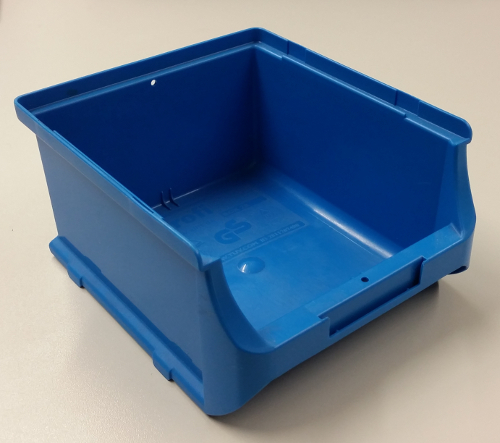
\includegraphics[width= 0.45\textwidth]{./images/container_blue.jpg}} \hspace{1cm}
		\subfloat[red]{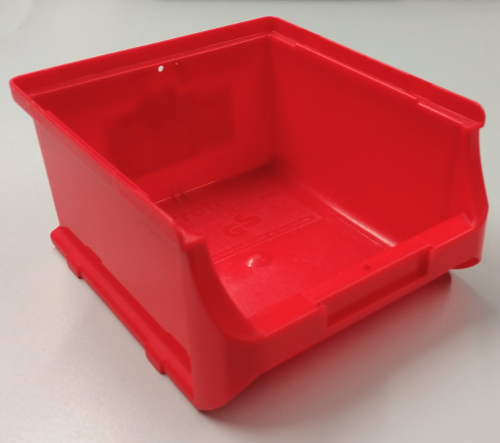
\includegraphics[width= 0.45\textwidth]{./images/container_red.jpg}}
	\end{center}
	\caption{Containers can be used for grasping objects out or placing objects into them.}
	\label{fig:containers}
\end{figure}


\subsection{Grasping Objects} \label{ssec:GraspingObjects}
If not specified differently in a test, the following definition applies to decide if an object counts as being grasped from a service area.
\par
An object counts as grasped from a service area, when the object was moved outside of the source service area. Outside means, that the vertical projection of the object’s convex hull does not touch the service area any more.

\par
The last point shall enable to let the robot pick up an object in order to analyse its type, e.g. by holding it close to a camera on the robot.
\par
If the robot handles an object, but does not fulfill all points above, the object does not count as being grasped, and neither points for grasping a required object, nor penalty points for grasping an unspecified object are given. Still, if the object drops to the ground or an uncontrolled collision occurs, the normal penalty points apply.

\subsection{Placing Objects on Service Areas} \label{ssec:PlacingObjects}
If not specified differently in a test, a manipulation object counts as placed on a target service area if any part of the object is touching the surface of the service area and the object is not moving at the end of the run. An objects does not count as placed when it is dropped (e.g. dropped from a height above 5 cm). This is to avoid that robots throw objects and potentially harm people or property.
\par
The pose of the object on the service area can be chosen freely by the robot.

%\section{Overall Scenario and Variation Points}
%The following two figures illustrate the kind of arenas that can be built with the previously described components. Figure \ref{fig:example_map} shows an old arena configuration (from IROS 2012) as a topological map defining places and connections, while Figure \ref{fig:example_map_go13} shows an arena configuration (from German Open 2013) with only a few surrounding walls, more open space and a conveyor belt.

%\begin{figure}
%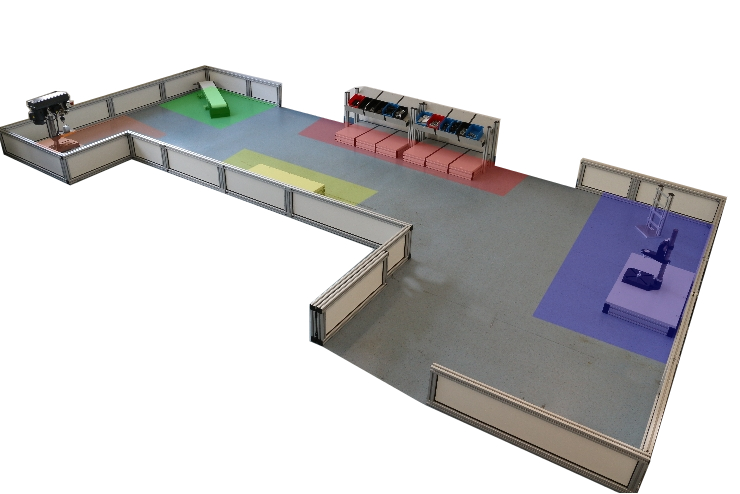
\includegraphics[width= \textwidth ]{./images/arena_brsu_spatial_areas.jpg}
%\caption{Illustration of one possible arena configuration. \todo{similar to Figure~\ref{fig:example_arena}. Delete one or put them together in a subfigure environment}}
%\label{fig:example_map_brsu}
%\end{figure}
